\subsection*{Viernes, 22 de Julio}

En este d'ia un poco nublado, me toc'o un avi'on c'omodo a Frankfurt.
\textexclamdown Qu'e emoci'on, por fin llegar a Alemania! Ir'iamos a Suiza para
despu'es virar al Norte y meternos en Alemania, es decir que no fuimos en
diagonal, y que vi cadenas monta\~nosas varias. Me sorprend'i volando a M'alaga
de ver un avi'on a lo lejos mientras nosotros 'ibamos en la misma direcci'on, en
comparaci'on esta ruta parec'ia una autopista: \textexclamdown cont'e 7 aviones
cercanos a nuestro vuelo! En uno me asust'e bastante: iba mirando alg'un lago
distra'ido, y pas'o \emph{\textexclamdown a fondo!} otro avi'on en sentido
contrario, poquito m'as abajo que nosotros. Se ve'ia grande y evidenciaba lo
r'apido que van estas m'aquinas, al pasar tan cercano. Uno ni se imagina la
velocidad, porque son m'as suaves que sentarse en un puf estos monstruos. Otro
se acercaba de costado y descend'ia para pasarnos por abajo. \textexclamdown Son
\emph{tan} grandes! Es muy tonto (mejor tildarlo de curioso) preguntarse esto,
pero me parece incre'ible el funcionamiento de los aviones. Es magia. Pasamos
monta\~nas, ciudades y lagos hermosos, un sue\~no, y vi un pico nevado sobre las
nubes bajas. Tambi'en se notaban varias pistas de aterrizaje desde el aire.

Bajando en Alemania se ve'ia todo perfectito. Los arbolitos, miles, todos en
fila india; las casas con techos a dos aguas, todas similares y de colores
ocres, marrones y amarillos; puentes y autopistas, trenes por todos lados,
barcos de carga en un gran r'io, este avi'on bajando, en fila con otros a este
gran aeropuerto. Todos {\small BMW}s (muchos ``rurales'', que all'a casi no
hay), Audis, {\small VW}, Mercedes, no muchos Porsches; todo prolijo, todo bien
hecho, todo lindo. No hay cosas que desentonen. Maquetas.

\emph{Toda} Alemania es verde, tupida. Voy a correr a un bosque cercano a la
casa, el camino es un t'unel de vegetaci'on por el que se filtran rayos de sol.
Lleno de subidas y bajadas que lo hacen m'as especial. Olv'idense de un camino
de 2~km sin curvas, eso no existe. S'olo en autopistas. Tengo bici para recorrer
las sendas, donde hay turbinas e'olicas. Parecen comentarios desprendidos, pero
sigue todo una misma l'inea: belleza y prolijidad por donde se mire y ande.
\textexclamdown Hasta el asfalto es m'as lindo! Yo no se porqu'e pero me gusta
m'as oscuro, y en Espa\~na era m'as claro. \textexclamdown Aunque si era al
rev'es seguro me gustaba el claro!

Al aterrizar tom'e primero un colectivo que me lleve a la parte 1 del aeropuerto
de Frankfurt, que es enorme. Compr'e un boleto de tren en esta zona 1,
\textexclamdown pero ni idea ten'ia d'onde tomarlo! Preguntando por aqu'i y
por all'a y caminando, llegu'e a un anden 1, pero subterr'aneo. Sub'i al tren
equivocado, obvio; lo tom'e antes por ansioso. \textexclamdown Pero le mostr'e
mi boleto a un alem'an puto y a las apuradas me dijo que era ese! Cuando no
ve'ia nunca la luz del d'ia y ve'ia que el nivel no se condec'ia con lo pagado
--y que paraba cada 100m-- me di cuenta de que no ser'ia\ldots\ pregunt'e, y la
se\~nora que se sentaba a mi lado me dijo que tome el subte (\textexclamdown en
un subte, no tren, estaba!) de vuelta, 4 paradas, y en ``Frankfurt Main'' mire
cu'al era mi tren; es decir que lo tomaba m'as adelante del aeropuerto y este
subte s'olo me llevaba a la estaci'on principal, \emph{Hauptbahnhof}. Menos mal
que pequ'e por temprano y no por tarde.

Llegu'e a la estaci'on y era m'as grande que el aeropuerto. Tenia \emph{seis}
minutos para la salida de mi tren desde all'i. Informaci'on estaba dos niveles
arriba. Sub'i corriendo por las escaleras con mochila y bolso, todav'ia me
pregunto c'omo llegu'e sin dejar las rodillas por el camino. Si tomaba las
escaleras mec'anicas la gente me demoraba, \textquestiondown y a qui'en se le va
a ocurrir usar las fijas? Al preguntar en Informaci'on, col'andome con permiso
y cara de ``llego tarde, \emph{\textexclamdown enschuldigung!}'', me quedaban 4
minutos pero era cerca: and'en 7.

Pregunt'e a una joven pareja ah'i mismo para confirmar, y contestaron que sale
del and'en 6.

\subparagraph{}\label{ssub:AngeldelaGuarda} --- \textexclamdown Pero en
informaci'on me dijeron 7!\\ --- Pero lo cambiaron a 'ultima hora.\\
\hangindent=1cm

Y les cre'i, porque ellos tomaban el mismo tren: pasaban G\"ottingen. Si nos
equivoc'abamos, nos equivoc'abamos juntos, y m'as vale eso que no estar seguro
solo. Una hora de viaje por valles, sierras, campos y fincas, parado en un tren
m'as suave que el avi'on; y despu'es de saludar a la pareja 'angel-de-la-guarda
cari\~nosamente, baj'e en mi nueva ciudad.

Taxi a la joyer'ia de Gustavo, y \emph{here I am}, por fin. De taxi un Skoda,
del nivel del Passat o mayor. Todos {\small TD}is. Yo no lo puedo creer.

Me instal'e, bien recibido por toda la familia (Gustavo e Ina, y sus hijos,
Pablo y Felipe). A cenar y descansar.

\subsection*{S'abado, 23 de Julio}

Hoy conoc'i a un amigo de Gustavo, ``Folka'', de unos 65 a\~nos. ``Folka'' es
una parte de su nombre, que empieza con ``\emph{Volks}''; significa hombre del
pueblo (y no, no existe el femenino de ese nombre). Sabe 5 idiomas
perfectamente, y me dej'o picando la posibilidad de visitar Turqu'ia en Agosto,
en un ``viaje de cultura''. Simp'atico el tipo, adem'as. Profesor de universidad
de idiomas y geograf'ia. Conduce un New Beetle negro descapotable. Viaj'o por
todo el mundo, a Gustavo y a mi nos ense\~na castellano y sobre cosas que hay en
Argentina, Chile, Per'u\ldots\ Y lo hace con buena onda, sin arrogancia. Juega
al tenis y lo lleva loco a Gustavo: ``todas a los pies''.

Al abuelo de Ina lo mataron en la II Guerra Mundial. No lo llevaron al frente de
batalla porque con su auto --uno de los pocos-- tra'ia v'iveres a la ciudad.
Pero alg'un nazi o cobarde denunci'o algo y lo llevaron a fusilar. Claro que es
la historia que ellos me cuentan no la del denunciante, pero es perfectamente
posible. Estoy leyendo ``Stalingrad''. Cada d'ia que pasa veo lo irracional que
son las guerras. Y cada p'agina del libro tambi'en me lo muestra.

Vi partes de la divisi'on Alemania comunista/federal. Me atosigaron con charlas
pol'iticas al verlo. Debe haber sido interesante, pero al no estar bien
instruido y le'ido no pude aprovechar la discusi'on.

Ayer a las 5pm est'abamos asando en la parrilla nueva de Gustavo. No sab'iamos
si almorzar o cenar (ac'a se almuerza tipo 3). Cre'imos que merendar'iamos pero
la sobremesa hasta las 8 nos indic'o que se trataba de una cena. Les ense\~n'e a
hacer matambre al lim'on. Como no existe el matambre Gustavo fue a la
carnicer'ia y le indic'o al comerciante que sacara una vaca para mostrarle qu'e
cortar.

Hoy comimos en un pueblo afuera de G\"ottingen, un restaurant ``t'ipicamente
alem'an'' seg'un Ina; delicioso todo. La cerveza ac'a me gust'o. No es helada.
No es tan amarga.

Volvimos por una ruta que pasaba cerquita de las turbinas e'olicas,
\textexclamdown su enormidad espanta! Despu'es vimos decenas de ovejitas,
dos perros, y un pastor. Era un encuentro de pastores, todos vestidos muy de
'epoca me pareci'o. Hab'ia cientos de autos, cientos de personas, y dos
chiringuitos vendiendo helados y cervezas. Me pareci'o un poco americana la idea
porque estaban todos en las mesas charlando y riendo, sin dar ni bolilla al
pobre pastor arreando las muchas ovejas. Eran la excusa para juntarse a tomar en
un prado. Los dos ovejeros alemanes corr'ian y ladraban, y el pastor con su
bast'on llevaba a todas las ovejas por donde quer'ia. Otro pastor ten'ia un
bast'on muy raro. Al preguntarle de qu'e se trataba, despleg'o dos palitos
formando una silla de cuero, y enterrando una punta se sent'o c'omodamente y
cruzado de brazos ante nosotros. \textexclamdown Pago en d'olares esa sillita
para mis viajes! C'omodo y divertido artilugio.

El BMW serie 5 de Gustavo pierde parte del encanto al enterarse uno de como lo
adquiri'o. Una mujer se lo cambi'o junto a muchos euros por un anillo y un
reloj. Es decir que esa \emph{m'aquina} vale lo que para una mujer dos joyas.
Que las personas somos diferentes no hay dudas. \textexclamdown S'olo Dios nos
puede llegar a ver iguales!

Aqu'i \emph{todas} las bicis llevan luces a d'inamo, que se dejan en las calles
porque no existe el robo, al menos en G\"ottingen. Y cada beb'e de cada edad usa
la sillita correspondiente para el auto, por seguridad ante posibles accidentes.
Aunque a veces, con tantos cuidados, se pasan del equilibrio me parece (no es
este el ejemplo).

Todos me dec'ian que es un lugar muy diferente Alemania, y no se equivocaban. Me
encanta.

\subsection*{Domingo, 24 de Julio}

Conoc'i hoy a tres parejas amigas de Gustavo: dos alemanas que no hablaban otro
idioma, y otra alemana que hablaba ingl'es, y el hombre es un fan'atico de todos
los deportes. Practic'o casi todos en serio, hasta esos saltos atl'eticos de
todo tipo que no conozco el nombre. Tiene una hija pre-adolescente m'as
vergonzosa que una paloma pergaminense, que quiere que aprenda castellano.
Porque ya habla alem'an e ingl'es (con 13 a\~nos) pero quiere que aprenda
espa\~nol para cumplir con facilidad los dos idiomas extranjeros obligatorios
que le exige la escuela secundaria. Ya hizo un viaje de intercambio estudiantil
a Estados Unidos que le gust'o. La otra opci'on era franc'es pero concluyeron
que no lo usar'ian tanto como al espa\~nol. Me comprar'ia, por ejemplo, boletos
en tren a \emph{Hannover} para conocer el zool'ogico y todo lo que tengo que
hacer es lograr que mantenga conversaciones en este idioma. Un poco ya sabe, no
ser'a imposible como cre'ia. Me pidi'o dos meses, todos los d'ias. Al terminar,
si todo anduvo bien, pagar'ia adem'as un viaje a Egipto para bucear en el mar
rojo (antes de Octubre).

\textexclamdown Viajar'ia a Egipto a bucear! Todav'ia Gustavo dice ``hay que
arreglar para que conozcas las pir'amides, todo''. Hay tiburones y ``\emph{all
kind of color fishes}''. Me ense\~nar'an buceo, mientras, en una pileta de
G\"ottingen. Ellos saben que yo vine a conocer cosas nuevas. Lo grande es que no
me dicen c'omo, \textexclamdown sino que adem'as me invitan!

Me contaba este hombre, Axel Becker, que viaja a Austria 2 semanas. Entonces me
deja su buena bicicleta todo terreno para andar por los bosques G\"ottingeanos,
mucho mas c'omoda y divertida que la de paseo que me presta Gustavo. Al final no
creo que la use mucho porque\ldots\ \textexclamdown me invit'o a pasar con su
familia y otra amiga a Austria! \textquestiondown Qu'e har'iamos en Austria dos
familias alemanas y un argentino? \textquestiondown Cu'al es el inter'es que los
une en un viaje? ``\emph{Wild Life} europea''. 8~km de un camino de piedras,
cerrado por una tranquera austr'iaca, hasta una casa sin electricidad ni
comodidades t'ipicas. Hay que buscar agua de vertiente, y bajar todos los d'ias
a un pueblo en bici a comprar el pan. Buena onda la familia, Gustavo asegura. 7
horas en una ``Touran'' (la van de camping de Volkswagen) hasta Austria. Hay
nieve, osos pardos (no los veremos seg'un dicen, espero Dios no los oiga),
ciervos (bambis), 2 vaquitas cerca de la casa, y otros bichos que ya no me
acuerdo. La casa es de un conde que tiene un palacio y grandes terrenos. Los
primeros tres d'ias los pasamos en el palacio como para compensar la falta de
comodidades de las otras dos semanas, que pretend'ian ellos asustarme pero son
las que me llaman a ir. Todos estos son proyectos, se llega a concretar alguno y
soy el hombre m'as feliz del mundo. Todo verde dicen, hay caballos, bicis y cada
uno se lleva sus piernas para recorrer. Espero que tambi'en algo para
protegernos, porque otro de los bichos eran ``\emph{wild pigs}'', jabal'ies.
Dicen que no son peligrosos, pero de eso no me f'io tanto. \textexclamdown Ya
les contar'e! Dicen que la sidra preparada por estos campesinos es riqu'isima.
Sino, la tendr'e que tomar igual porque hay pocas opciones, pero todo ser'a
casero.

En este encuentro sali'o un viaje a Egipto, otro a Austria, y curso de buceo;
sin mencionar que el asado argentino se celebr'o en Alemania. Turqu'ia, como ya
dije, era muy loco y voy ``invitado'', no invitado. Entonces no me alcanza el
dinero, o s'i pero para nada m'as. Esto es ``\emph{all inclusive}''.
\textexclamdown De todos modos mucho no voy a gastar en Austria porque no hay
donde usar plata! Ma\~nana voy a trabajar a la agencia de viajes del loco (solo
de viajes de buceo, vean qu'e especificidad) para terminar un sitio web de
Argentina antes de desenchufarme del mundo. Las compus de Gustavo son malas
excepto la mejor del mundo, que est'a en la vidriera de la joyer'ia por poco y
no la puedo usar. Desenchufarme en Europa me suena contradictorio.

Cuando Gustavo me lo present'o, dijo: ``se llama Axel, como Blumberg''. Sigue
las noticias argentinas el loco.

Una de las primeras cosas que le cont'e fueron mis viajes y proyectos de viaje
en bici (qu'e iron'ia, con proyectos ac'a). Esto ya parece medio loco tambi'en,
pero me dijo que podr'ia trabajar en su agencia para integrar cicloturismo (y no
trabajar solo buceo). Con contarles mis viajes, ense\~narles cosas, armar un
posible viaje de los que ya hice estar'ia adentro. Dios quiera que salga,
\textquestiondown se imaginan qu'e placer m'as grande ganar \geneuronarrow{1}
por contar mis viajes o proyectar? \textexclamdown Si fuera lucrativo vivir'ia
de eso en Argentina! Adem'as necesito actividades en esta vida ac'a. Aunque si
salen todas, de verdad no me alcanzar'a el tiempo. Una de las parejas alemanas
eran capas en la universidad y ver'an la posibilidad de ir a estudiar el idioma,
4 horas todas las ma\~nanas. Muy bueno, interesante.

\subsection*{Lunes, 25 de Julio}

Hoy a la ma\~nana pase'e en bici por G\"ottingen. Me dieron ganas de sacarle una
foto a'erea al cruce principal. Hay bici sendas por muchos lugares, y este cruce
es una obra de arte. L'ineas blancas por todo el asfalto, veredas con colores en
el piso para separar peatones de ciclistas, y dos sem'aforos de cada lado:
peatones y bicis, y autos. Ac'a se usa mucho la bicicleta, y es hermos'isimo
verlo. Si vieran qu'e nudo mas complejo parece, y c'omo organiza r'apida y casi
m'agicamente a este enjambre de veh'iculos entender'ian lo perfectito que se ve
todo. Es como las im'agenes de ciudades que repart'ia el ``Billiken'', todo
perfectito. \textquestiondown O ser'a que estoy de vacaciones? No se ven esas
cosas comunmente all'a, porque no hay bicis, de las que hay no son respetadas
como medio de transporte alternativo. Y 'estas tampoco respetan al no ser vistas
de noche, o por no tener patentes que identifiquen. \textquestiondown El huevo o
la gallina?

Despu'es dorm'i una peque\~na siesta porque llov'ia, y al despertar estaba
soleado. Sal'i a correr al bosque, antes de que se vuelva a largar (a la noche
lo hizo). Corr'i bien creo, pero las subidas y bajadas no me permiten comparar
con lo que hago en Argentina. Bajando trabajan las rodillas, y subiendo el
coraz'on, que me pide m'as aire que el que hay en todos los bosques. Pero
justamente estos accidentes geogr'aficos hacen que quiera llegar ``hasta la otra
curva y nada m'as'', para ver qu'e hay del otro lado y se repite en cada curva.
Y siempre encuentro lo que esperaba: belleza natural. Despu'es de la lluvia
hab'ia un olor a tierra mojada que parec'ia energ'ia para correr. Aire
\emph{fresco}. Los caminos son anchos, pero se puede tomar los internos que se
meten entre los 'arboles y tienen el ancho de una bici.

Reci'en comimos un terrible asado. Les gust'o la idea del lim'on en el
\emph{killhungry} (``matambre'', ac'a la traducci'on se hace directa).
Ensaladas de todo tipo, tienen tantas cosas raras que no puedo creer que sean
ricas. La mesa era un desorden: tres idiomas hablaba Gustavo y yo trataba de
seguir mi ingl'es. No s'e como las otras dos parejas alemanas no se enojaron:
casi nunca se integr'o en ese idioma. Simp'aticos todos.

Axel me contaba (sobre el tema que siempre llamar'a mi atenci'on) que despu'es
de la Segunda Guerra Mundial sigue el {\small NPD} y grupos neonazi. No los
pueden censurar por la Constituci'on, pero a diferencia de lo que yo pensaba son
menos del 5\% del pa'is. Le dije que me parec'ia una locura de gente, pero
contest'o que siempre hay locos para todo, y que ``mientras sean poquitos los
podemos contener''. Todos los alemanes (dec'ian 'el y Gustavo), son dem'ocratas,
o republicanos, o lo que sea el {\small SPD} que es el que ahora gobierna.

\subsection*{Martes, 26 de Julio}

En estos barrios el mundo parece perfectito en serio, y chocan los mails del
diario por eso. Claro, es que \emph{este} mundo se acerca a lo que llamo
``perfectito''.

A la ma\~nana fui a las oficinas a hacer unas cositas. Axel me invit'o a
almorzar y despu'es unas gu'ias tur'isticas de la agencia me mostraron un poco
G\"ottingen. Me mostraron una edificaci'on del a\~no 1412. Y varias casas tan
vencidas que dan ganas de quedarse haciendo fuerza para evitar el derrumbe.
Pasamos por un restaurante ``espa\~nol''. Todo lo que ten'ia de espa\~nol era el
men'u, porque la imagen era claramente norteamericana, con algunos indios
mejicanos.

Y a la tarde, \textexclamdown por fin cac'e la bici nueva! Es una m'aquina, m'as
c'omoda que la m'ia (el cuadro m'as grande la hace mas c'omoda, aunque menos
``canchera''), y con cambios m'as r'apidos y precisos (\textexclamdown a'un!).
Me emocion'e, y al llegar a casa cambi'e los pantalones y sal'i al bosque. Para
conocer m'as, en vez de doblar y volver a casa, segu'i el camino derecho.
Despu'es de cruzar todo el bosque llegu'e a las turbinas e'olicas. Me asustaba
un poquito primero por el t'unel del bosque, que hace que no se vea a un metro
de distancia, estando solo en un camino poco transitado. Despu'es, no se porqu'e
(como algunos a los payasos, sin raz'on aparente) pero de cerquita ver esas
turbinas girando tan despacito y tan inmensas, me daban un poco de respeto
tambi'en. No pod'ia pasarlas como por al lado de un poste, las vigilaba como un
perro al caballo. Es raro. Es lo mismo que siento cuando pasa un avi'on de esos
de publicidad mientras estoy dentro del mar en Mar del Plata, hay algo en eso
que me desespera.

Agrego para la ing. qu'imica de Espa\~na que las turbinas e'olicas son
\emph{muy} silenciosas. S'olo se escuchaba mi respiraci'on y los cultivos
mecidos por el viento. \textexclamdown A no andar usando razones inveros'imiles
para apoyar la energ'ia at'omica!

Llegu'e a un pueblito, donde tom'e un camino de campo. Las subidas y bajadas y
curvas entre trigo y girasol, y c'omo se ven los tejados a dos aguas de pueblos
lejanos entre las sierras, son de f'abula. Llegu'e a otro pueblo, y ya quer'ia
volver. En 6~km cruc'e tres pueblos, \textexclamdown igual que en los caminos de
Pergamino! Volver'ia por el mismo camino (imposible volver a encontrarlo
despu'es de tantas bifurcaciones, adem'as ya lo conoc'ia) o describiendo un
circuito. No anduve mucho, unas 2 horas, pero a la hora ya me empieza a
interesar saber donde estoy. Di una vuelta enorme, y describiendo una ``V''
corta volv'i a las mismas turbinas e'olicas, pero ahora ve'ia la ruta con
carteles a G\"ottingen. \textexclamdown Y los techos que vi en todo el camino
eran los de la ciudad que buscaba, que cre'i estaba del otro lado de los
bosques! Es decir que el camino por bosques est'a lleno de curvas que no cont'e,
y hace parecer mucho m'as largo un mismo recorrido. Ahora, a conocer siempre que
pueda, aprovechando los pocos d'ias de buena bici.

La bici tiene 8 pi\~nones, 24 cambios. En algunas bajadas los tiraba a todos y
iba realmente \emph{r'apido}. Al tocar los frenos se sent'ian tan suaves aunque
potentes, como una moto que pesa 10~kg. Ese es el placer de las bicis. En
las curvas cerradas en pavimento en bajada se escuchan los tacos de las
cubiertas todo terreno. \textexclamdown Y la vegetaci'on de los costados
magnifica la sensaci'on de velocidad! Gracias, Axel.

La pr'oxima espero volver a perderme, porque ac'a todo es cerca. Y saber que
est'as perdido, que parece que est'as lejos, pero que en media hora pod'es estar
de vuelta en casa se siente bien. Para dar una idea, lo que hice hoy es como
llegar a Arroyo Dulce desde Perga (sin la vuelta), pero cruzando 4 pueblos. Y
tres turbinas e'olicas: una grande y lenta, y dos m'as peque\~nas y r'apidas. Si
estoy perdido alguien me va a ubicar entre tantas peque\~nas poblaciones. Todo
el mundo habla ingl'es, y todos se excusan de que lo hablan ``\emph{a little
bit}''.

Ma\~nana me espera un d'ia similar, y con confirmaci'on de Austria.
\textexclamdown Qu'e aburrido, un d'ia similar!

\subsection*{Mi'ercoles, 27 de Julio}

El no parar de mover las piernas y el clima pesado me llevaron a quedarme en
casa, as'i que le'i, dorm'i, y anduve poco en bici por la ciudad. Les cuento que
en Austria ``el palacio tiene solo dos habitaciones armadas'', as'i que no puedo
ir. Triste, pero igual no era planeado. Axel me pregunt'o si quer'ia
``cambiarlo'' por Egipto. ``\textexclamdown Pero era un regalo!'', contest'e.
As'i que tengo dos semanas de bici sin parar. Despu'es saldr'e a correr,
mientras la aprovechar'e.

Hoy visitar'e alg'un bar G\"ottingense para ver qu'e onda. Aunque quienes me
llevan son aficionadas al hip-hop, calculo que en el bar un Mi'ercoles ser'a
m'as tranqui la onda. Son quienes trabajan en la agencia de viajes, la semana
que viene hacen el mismo viaje a Egipto. Tienen que viajar por trabajo, para
conocer el producto que venden. \textexclamdown Muy buen trabajo! Veremos
qu'e cuentan cuando vuelvan, la siguiente semana.

\subsection*{Jueves, 28 de Julio}

Hoy me levantaron no muy tarde para ir a Kassel, a un complejo tur'istico muy
grande de termas y cosas de relajaci'on. Menos mal que fuimos, porque sino, con
el estr'es que vengo acumulando muero. Fuimos la familia menos Ina, que trabaj'o
en la joyer'ia. Todo muy bueno: jacuzzis, todas las piles climatizadas y con
sales; me met'i en un sauna y todo. Est'a bueno porque hace transpirar todo el
cuerpo. Uno juega al tenis y transpira casi todo, pero en el sauna se transpira
el 100\% de la piel. Con ``aromaterapia'' que recordaba al living de casa. El
cartel dec'ia ``80 a 90 grados''. Parece que quemara al entrar pero no. O debo
ser \emph{re}bruto y lo deben medir en otro lado. Seguro. Solo al salir queman
los pies, que sino descansaban sobre la toalla. \textexclamdown Es divertido ver
a la gente salir corriendo!

El nudismo no es cosa del otro mundo. Entonces no se para qu'e se sacan todo,
seguro encuentran alguna raz'on que desconozco. Cuando es tan natural uno
ni se da cuenta, es casi lo mismo s'olo que se ven partes m'as blancas del
cuerpo. \textexclamdown Cuando me vaya de Alemania seguro el Gobierno me vuelve
a invitar para volver a embellecer Kassel!

En la pile de afuera se ve'ian aviones cada dos por tres, y los caminitos de
nube que van dejando, cruzados o paralelos. Se nota que Alemania es transitada
all'a arriba, un piloto ac'a debe tener poco tiempo para tomar mates.

Seguimos paseando por Kassel despu'es de las termas, y llegamos a un palacio.
Los chicos estaban muertos en el auto pero quer'ian bajar porque ve'ian a ``los
grandes'' hacerlo. Se ve'ia un camino todo verde que era pasto importado
de Inglaterra para m'i, que sub'ia un gran cerro (lleno de gente) hasta llegar a
un antiguo y gran castillo, lejaano lejano. Bajaban dos bicis de descenso (esas
que parecen moto-cross por forma, precio y velocidad), calculo que la sonrisa
no les entrar'ia en el casco a los ciclistas. \textexclamdown Qu'e diversi'on!
Andar as'i, por un lugar sin camino. Pero no lo visitamos hoy, porque los chicos
estaban inquietos.

En vez de volver por la autopista, lo hicimos por la ruta vieja. Paramos en un
pueblo muy antiguo, \emph{Hann-M\"unden}. Todas las casas son del siglo {\small
XV} o {\small XVI}, y la mayor'ia est'an vencidas; hay una capilla grande hecha
con piedras de todo tama\~no, otra iglesia m'as grandota con un techo alt'isimo
y un campanario original, un puente que cruzaba un r'io muy bonito lleno de
patos y ``una garza gris con pico rojo'' (el patito feo entre todos los patos).
Sobre este r'io se proyecta toda la vegetaci'on, y un palacete relativamente
moderno. Las mesas en la calle invitaban a un chocolate caliente. Gustavo sac'o
una foto a una fecha pintada en una casa: ``1657'', y no era la m'as vieja. Le
pregunt'e para qu'e, y era para comparar la historia de una antig\"ua
civilizaci'on, con la de Argentina, en una peli que est'a haciendo.

\textexclamdown Hasta las gr'uas de la construcci'on son menos feas por aqu'i!
No son en forma de ``T'' sino de ``L'' invertida, m'as bonitas, con tensores
diagonales. Los pesos van abajo, no arriba.

Seguimos viaje, y la ruta se torn'o tan angosta que cre'i que era de un sentido.
\textexclamdown No se c'omo se animaron unos ciclistas que adelantamos a
tomarla! El camino lleno de curvas no nos llevaba a G\"ottingen porque el
desv'io estaba cerrado por reparaciones. Preguntando llegamos a un ferry que nos
cruzar'ia por el r'io hacia otro desv'io. No se ve'ia motor: cruzaba con la
energ'ia de la correntada, sostenido por dos sogas a un cable transversal,
simpleza total. Ese debe estar bueno para que lo conduzcan las mujeres:
\textexclamdown solo puede chocar con dos riberas de pasto!

El ``be-eme'' serie 5 parece ser una m'aquina placentera en las rutas, pero
despacio no se nota, y fuerte no me animaba a disfrutarlo. Es un 6 cilindros y
ruge como un motor grande. Gustavo se quiere comprar un Laguna, \textexclamdown
pero comprar un importado en Alemania es una paradoja! Comprar importados all'a
en Argentina es comprar todos, pero entre lo ``grande'' es comprar alemanes
creo. Dice que dentro de Alemania la de m'as prestigio es Audi. Pero la verdad
es que los rurales {\small BMW} son m'as bellos. L'astima que no hay con
tracci'on integral.

Ahora tengo planeado irme con bici (se suben en el tren) a Kassel, separado por
unos 50~km, para recorrer bien todo lo que qued'o. La vista hacia abajo desde
all'a debe ser indescriptible.

Siguiendo con ``proyectos raros'', Gustavo est'a viendo la posibilidad de dar
una vuelta en globo aerost'atico. \textexclamdown Tiene cada amigo que me hace
morir de risa!

Es impresionante c'omo cambia el clima en un d'ia. Anoche hubo lluvia y tantos
rayos (sin sonido: ``que van de nube en nube'') que me daba cagazo dormir.
Duermo bajo un ventanal. Hoy, sol pleno. Y esta noche, \textexclamdown tormenta
m'as ventosa y ruidosa que la de ayer! As'i se mantienen los bosques verdes, y
el sol en la tarde para disfrutarlos. Sincronizaci'on perfecta hasta ahora.

\subsection*{Viernes, 29 de Julio}

Hoy fue incre'ible. Me levant'e temprano con tormenta. Toda la ma\~nana y
almuerzo: sol, las chicas en la agencia de turismo me preguntaban qu'e hacia de
pantal'on largo. Me acost'e media hora despu'es de almorzar, para salir luego a
andar en bici, pero ahora llov'ia. Una hora despu'es par'o, y no lo dud'e, las
nubes no amenazaban demasiado. Sal'i, esta vez con c'amara de fotos. Me
invitaron a una pile pero prefer'i pedalear por lugares nuevos, \textexclamdown
hice bien!

Tom'e otro camino, como estaba tan mojado no pude acelerar mucho en las bajadas.
En pocos minutos estaba en un cruce conocido, que cre'ia lejano. Es f'acil de
perderse en caminos boscosos. En media hora estaba en las mismas turbinas
e'olicas que antes de ayer hab'ia visto a la hora de pedalear. Y el mismo
pueblo, \emph{Diemarden}, poco m'as abajo. Estuvo bueno porque pedaleaba por ese
t'unel todo oscuro de vegetaci'on, que no se ve por donde sigue el camino, y
``redepente'' llegu'e a un claro, un cultivo de trigo. A mi derecha por el
camino acompa\~naban los bosques, y al terminar la cortina verde aparecieron de
golpe y cerquita las turbinas e'olicas y casi me da un espasmo. Por suerte a la
vuelta me amigu'e y me puse al lado para apreciar su tama\~no (estaban paradas).
Por los pueblos hice un mont'on de fotos que parecen postales, pero no por
m'erito del fot'ografo sino de la Naturaleza que rodea.

No me gustaba la idea de seguir por los mismos caminos pero hab'ia llegado sin
querer, as'i que tom'e otro desv'io, de esos que por ac'a abundan: un camino que
se abr'ia, todo poceado y viejo, oscuro por la vegetaci'on. Parec'ia que llevaba
a lo que llamamos all'a un casco (ac'a no existen las ``estancias'' calculo)
pero un cartel indicaba que a escasos 2~km hab'ia un pueblito. \textexclamdown
20 cuadras y otro poblado! Los 2~km fueron de subida, y arriba de la colina
esperaban dos grandes techos: eran establos y de eso se trata \emph{Bettenrode},
solo equitaci'on. Hermos'isimo. Cuando llegu'e les mostr'e las fotos a Gustavo e
Ina porque no lo conocen, \textexclamdown las ventajas de la bici! En Argentina
viajamos en bici para ver cada detalle, pero ac'a para ser tan detallistas
habr'ia que caminar.

Despu'es de mirar un poco esto, segu'i el cartel de bici senda que indicaba
un camino que parec'ia privado pero que era ``p'ublico'', entre comillas porque
parece muy poco usado. Lo segu'i para ver qu'e hab'ia, y despu'es de una curva
la encontr'e: la bajada de la colina. En todo el viaje se ol'ia la tierra
mojada; se tienen tantas sensaciones juntas, durante tanto tiempo. El tema de la
bajada es que tambi'en estaba cubierta por 'arboles y arbustos y por tanto muy
barrosa, llegu'e a abajo todo sucio. De nuevo me sorprendi'o el final de este
camino: bajando por aqu'i y por all'a, r'apido, oscuro en la vegetaci'on,
apareci'o un techito de esos t'ipicos alemanes, antiguos. Yo, creyendo que
estaba llegando a una casa s'uper antigua que no conoc'ia ni el due\~no,
aceler'e. Al llegar se acab'o todo el bosque y sent'ia de nuevo el sol. Era un
pueblo que estaba a\ldots\ \textexclamdown 10~km de G\"ottingen! \textexclamdown
Y yo pensaba estar el doble de lejos! Ah'i estaba la ruta, \textexclamdown es
que uno no se puede alejar, ac'a! Y sin embargo \emph{siempre} hay cosas nuevas.
El camino desembocaba en una capilla del 1730, alta sobre una gran roca.

Segu'i por la bici senda a otro pueblo que estaba a 1,6~km para el otro lado.
Pensar que en Pergamino hago 50~km para ver Fontezuela, la Olla y si tengo
suerte unos b'uhos, y por aqu'i cada 20 cuadras aparecen pueblos, bajadas,
subidas\ldots\ Este pueblo era puramente campesino. Lleno de establos, vacas,
se\~nores que usan jardineritos, tractores, y una capilla con un peque\~no
monumento a los ca'idos en las guerras mundiales. Para mi los libros para
ni\~nos se escriben ac'a.

Al volver al pueblo de la capilla alta en la roca, el cartel de bici senda
indicaba G\"ottingen a 21~km, aunque por la ruta se acortaba a 11~km. Obvio
quise tomar la bici senda, pero a los 5~km desemboc'o de nuevo en la ruta y no
la pude seguir. No s'e porque la perd'i. Es dif'icil querer volver a casa porque
siempre se quiere seguir ``un poquito'' m'as hasta el ``'ultimo'' pr'oximo
pueblo, que es siempre pen'ultimo. Al volver se abr'ian caminos desde la ruta
que llevaban a las turbinas e'olicas, paradas seguramente por poco viento.
Hab'ia autos abajo y pude comparar el tama\~no: inmensamente grande. Y eso que
'estas eran las ``chicas'', la ``grande'' era inmensa de verdad. Se usan
camiones completos para transportar s'olo las aspas (imaginen: el radio es del
largo de un cami'on con acoplado).

Llegu'e y com'i todo, como siempre. Chocho de haber encontrado esto. Seguir'e
conociendo estas semanas de bici buena. Cuando la devuelva empezar'e a viajar en
tren seguramente. \textexclamdown Podr'ia visitar varias terminales
automotrices! Y conocer la Selva Negra.

Ma\~nana voy a jugar tenis, dobles con Gustavo; contra Folka, y un tipo al que
le salv'o la vida Gustavo. Lo vio tendido en la calle con un paro card'iaco y le
empez'o a empujar fuerte en el pecho, luego le hizo respiraci'on, y ahora vive.
\textexclamdown Estaba muerto! Me dieron ganas de aprender eso, se debe dictar
en la Facultad de Medicina. Es reanimaci'on, en la escuela me lo ense\~naron
pero se imaginar'an c'omo me acuerdo. Cada vez reniego m'as de la bastante
precaria educaci'on en mi escuela. \textexclamdown Pero c'omo la agradec'i, de
estudiante!

\subsection*{Lunes, 1 de Agosto}

El s'abado fuimos a jugar al tenis. Nos alegr'o que Pergamino no viera a sus
representantes en este mini torneo porque nos limpiaron r'apido. \textexclamdown
Qu'e lindo tenis tengo! (No traje abuela, che.) L'astima que juego tan poco. La
misma excusa se le ocurri'o a Gustavo. Pero estuvo muy lindo, un gran d'ia de
sol fue. Mi rev'es es para encuadrarlo y colgarlo en el living. Pero no
entrar'ia porque se van largas todas las bolas\ldots

Cenamos un asado de tira bien salado, en la parrilla que Gustavo hizo con
piedras tomando la nuestra de modelo. Tangos de fondo y todo. Cenamos con una
pareja de argentinos de padres alemanes. El hombre, Cristian, tambi'en tiene
como ultimo sue\~no al jubilarse volver a Argentina, ``a donde sea en la
Cordillera''. Ve'ia m'as los puntos negativos de Alemania. Al menos vino con
familia.

Vino el ``capo'' de la Facultad. Me dej'o una tarjeta que me habilita como
estudiante a comer por \geneuronarrow{2} en los comedores universitarios. No
puedo empezar clases porque est'a cerrado por vacaciones. Una l'astima, pero si
quiero disfrutar del verano\ldots\ \textexclamdown ``Sprechen Sie English?'' es
todo lo que necesitar'e! Que l'astima no pueda charlar con este tipo de la
universidad, parece tan simp'atico y se nota que intenta ayudarme. Adem'as debe
ser interesante su ocupaci'on. Siempre le agradezco, aunque nunca se muy bien
porqu'e.\\

Ayer Domingo fuimos en bici con Gustavo a una pileta a 13~km de casa, aunque de
ida hicimos 20~km porque al hacerlo investigar, nos perdimos. No hab'ia mucho
interesante durante el camino porque se ve'ia siempre lo mismo, es terreno
plano. Pero llegar a cada pueblo era una gloria, \textexclamdown todos son
lindos! Y mientras m'as en la colina est'en, mejor. Gustavo lleg'o muerto,
acalambrada hasta la nariz. Apenas llegamos empezaba una llovizna, as'i que,
luego de un rico helado, pegamos la vuelta. Hice una bajada a fondo, y lo
esperar'ia abajo. Era larga, cre'i que le hab'ia sacado un buen trecho. Cuando
yo no daba m'as empec'e a desacelerar\ldots\ \textexclamdown y el guacho me
empez'o a tocar su bocinita desde cerca! Desde ah'i, \textexclamdown 13~km de
carrera hasta casa! \textexclamdown No ven'ia tan acalambrado entonces! Muy
bueno el viaje, volvimos r'apido de verdad entre la bajada, y el viento antes en
contra ahora a favor. Est'abamos muy cansados pero en esas condiciones cualquier
cambio se tiraba solo, divertido. Sacamos varias fotos, sobre todo en un laguito
de G\"ottingen que ``en invierno se congela y se tiran en trineo'', y ahora en
verano tiene patos navegando.

Llegamos, y a estirar un poco los m'usculos\ldots\ nunca lo hice luego de la
bici, pero juntos hicimos fuerza todo el camino.\\

Y hoy, d'ia de descanso, con lectura y alg'un paseo por la ciudad. Ma\~nana a
las 6am empieza una jornada de entrenamiento con Gustavo de bicicleta por el
bosque, que en teor'ia tiene que durar un mes, a 3 o 4 veces por semana. Llueva
o no, porque si s'olo lo hacemos en d'ias de sol nos queda la mitad del
entrenamiento. As'i llega a Kassel a pedal. 30~km los hizo de un saque, en un
mes podr'a yo creo. El tema es la vuelta, pero al estar obligado, aunque no
podamos, podemos; sea caminando o pedaleando. \textexclamdown Nos esperar'a Ina
con dos asados juntos! Espero que dure esto, yo tengo ganas.

\textexclamdown Un fin de semana tranquilo!

\subsection*{Jueves, 4 de Agosto}

Como ya saben ayer iba a ser d'ia de entrenamiento con Gustavo, pero en la cena
anterior no se qu'e bicho me pic'o y quise ir a Kassel en bici. Lo decid'i el
d'ia del descanso, claro. Me mostraron un mapa con todos los caminitos que pueda
haber para bicis y autos, y me levant'e temprano para ducharme,
\emph{desayunar}, y salir tipo 8:30 am. Llegu'e de vuelta a casa a la misma hora
pero de la tarde, entre bici y paseo. \textexclamdown Doce horas! Queda a 48~km
por ruta 3, para autos y m'as directa. Por eso creo que pas'e los 100~km.

Saqu'e fotos a todos los carteles de pueblos que cruzaba, para contarlos y
acordarme. La primer perdida respecto al mapa fue en un cruce entre un camino de
tierra, y cuatro pavimentados. Perderme consisti'o en llegar a otro pueblo y no
al que quer'ia, pero de todos modos me acercaba a Kassel.

Anduve bastante hasta encontrar el r'io que empezar'ia a bordear al llegar a
\emph{Hann-M\"unden}, y un rato despu'es, tipo 12, vi un buen restaurante en la
ribera. Del otro lado del r'io hab'ia otro pueblo con un campanario de iglesia
hermoso. Lo dud'e un poco porque era temprano pero era el lugar m'as lindo, as'i
que par'e a almorzar. La mujer no hablaba ingl'es, le indiqu'e que por favor
trajera lo que estaban comiendo en una mesa cercana. \textexclamdown De todos
modos decir ``milanesa'' o ``bife'' en ingl'es tambi'en me hubiese complicado! A
la salida quer'ia agradecerles la elecci'on, era riqu'isimo. Primero una
ensalada de esas alemanas con porotos, verduras y crema de leche muy sabrosa.
Despu'es, milanesa con papas fritas. Com'i en una galer'ia donde las moscas no
molestaban porque iban al plato de entrada, y donde un gorrioncito pasaba a
fondo cada dos por tres al lado de mi cabeza. Tambi'en lleno de mariposas
blancas, que iban a una maceta con flores amarillas cercana. En el r'io se ve'ia
un patito nadando y durante un rato un cisne; una poes'ia de lugar.

Mientras tanto pasaban por el camino cientos de bicicletas. Se ve que es un
camino que se usa mucho por lo hermos'isimo que es, y por la cercan'ia a una
ciudad grande como Kassel, que a 10~km estar'ia. Despu'es de llenarme con
tama\~no plato\ldots\ \textexclamdown no pod'ia seguir ni empujando la bici!
Pero no me cost'o mucho esfuerzo digerirlo, me sorprend'ia lo grande del cuerpo
humano. Miren la estupidez que pensaba, pero, \textquestiondown se imaginan
tener que trabajar conscientemente para digerir? \textexclamdown Qu'e buenos
pensamientos surgen luego de horas de ejercicio f'isico!

El camino a Kassel fue divino. Una senda techada por 'arboles, el gran r'io con
frondosa vegetaci'on en las riberas, la ruta tras una pared de 'arboles y
arbustos a la derecha, y al otro lado del r'io, y tambi'en tras una pared de
vegetaci'on, las v'ias del tren que se escuchaba y no se ve'ia. Estos 10~km tuve
sobre mi cabeza a dos aviones caza, esos de a lo sumo dos plazas, \emph{muy}
r'apidos, haciendo piruetas y persigui'endose. 4 horas despu'es, a mi vuelta,
segu'ian, seguro un entrenamiento. Eran ``avionetas'' potentes, no sonaban ni a
motor convencional ni a turbina, por ah'i sea ``turboh'elice''. Tambi'en pasaban
aviones de pasajeros cada dos por tres y un helic'optero; parece una
enciclopedia de transportes.

Cuando vi por primera vez, all'a lejos y arriba de una colina, al H'ercules,
casi muero. Faltaba, pero ya casi estaba. Pregunt'e muchas veces c'omo llegar, y
nadie escondi'o su sorpresa al verme querer hacerlo en bici: todos me indicaban
los tranv'ias 1 'o 3. Alimentaban mis ganas de llegar, igual no era tan cansador
como lo pintaban. Ped'i agua (aprend'i la frase en alem'an, \textexclamdown si
no responden con una pregunta ando de diez!), hasta ah'i hab'ia tomado poco
andando regular y con refrescante viento. Pero en subida y sin aire transpir'e
todo lo que pude, las botellas parec'ian evaporarse.

El parque donde est'a el palacio y el H'ercules m'as arriba es un sue\~no, con
mucho pastito verde y perfecto, lleno de caminos y laguitos, muchos 'arboles,
todo prolijo; patos, cisnes, mucha limpieza. Empec'e a subir todo lo que pude en
la bici, haciendo eses por ese pastito y por caminos paralelos. Al llegar me
saqu'e una foto en la base de las escaleras del H'ercules (\textexclamdown
todav'ia escaleras!), y las empec'e a subir trotando con bici al hombro, porque
me pidi'o Axel ``\emph{take care of it}''. Si me pidi'o cuidarla de robos,
cumpl'i; si es no ensuciarla y usarla poco\ldots\ \textexclamdown con sonrisa
digo que no!

Dej'e la m'aquina a mitad de camino, en una galer'ia donde la pudiera cuidar, y
segu'i subiendo pisos y disfrutando miradores. Es impactante la vista desde
all'a. En una galer'ia creemos estar viendo tanto y tenemos v'ertigo,
\textexclamdown y al subir a la siguiente se ve tan bajita la primera!
Impresiona. Subir, subir y subir hasta esa cosquilla que dice ``\textexclamdown
basta!'' en gl'uteos y pantorrillas. Sub'i hasta donde m'as se pod'ia, pagando
\geneuronarrow{2} para entrar a la construcci'on, que ya s'i me asustaba por lo
alto. Vieja, sostenida por metales ahora. Aqu'i me daba tanto v'ertigo asomarme
por las terrazas (aparte de toda la colina, la verticalidad de la construcci'on)
que no me acerqu'e demasiado. Recorrer adentro y ver la vista a trav'es de las
ventanas, fue muy interesante. Pensaba en quienes subieron la cabeza a la
estatua del H'ercules y me temblaban las piernas.

Y ahora, la bajada. Al bajar las escaleras de este edificio vi, del otro lado,
la ruta por donde suben los colectivos tur'isticos, tan distinto al boscoso
camino que acababa de conocer. \textexclamdown Lindo choque creaba este
zaparrastroso tan transpirado entre los turistas tan pitucos! Transpirar as'i
hace sentir bien. Bajar las escaleras tampoco fue tarea f'acil, ahora la
cosquilla se presentaba en la parte delantera de las piernas. Lo debo haber
hecho r'apido y emocionado por llegar al camino para bicis, porque no recuerdo
c'omo hice con la bici, que tanto molest'o en las escaleras de subida.

\begin{center} 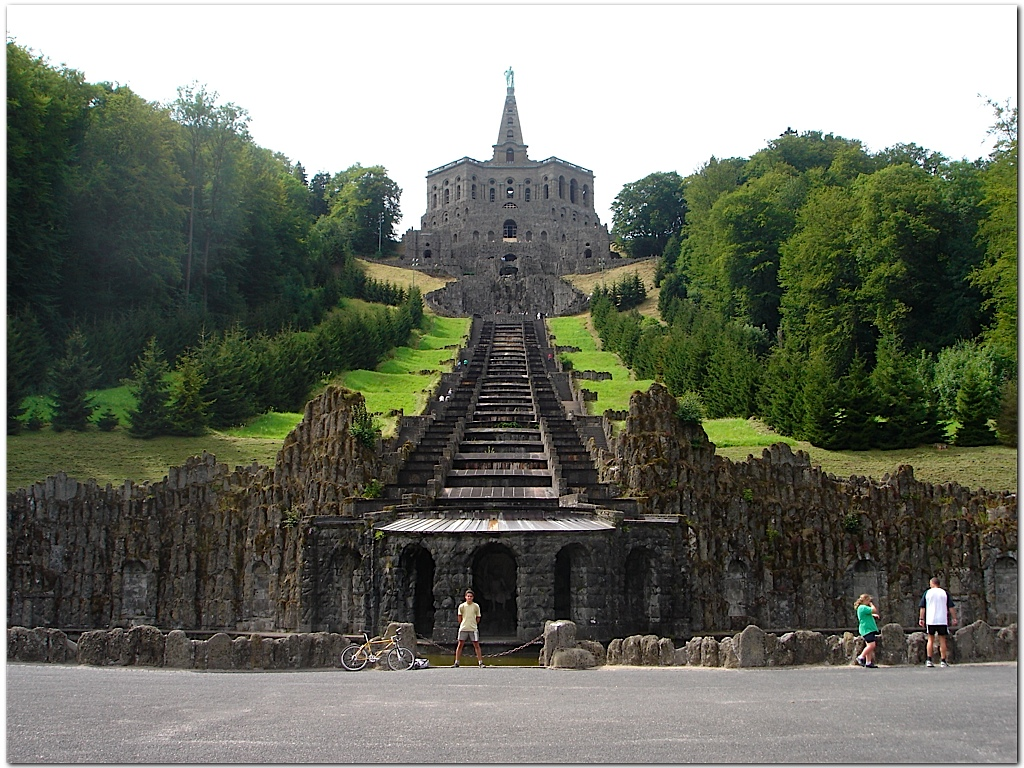
\includegraphics[width=300px]{images/DSC01248.jpg}\\ \textsc{Al
final de la colina, las escaleras al H'ercules.} \end{center}

Cuando llegu'e a la ruta entend'i porqu'e es mejor llevar bien infladas las
ruedas. \textexclamdown Iba muy r'apido, y las curvas se cerraban antes de que
las pudiera doblar! Las intentaba cerrar pero la bici se abr'ia solita, ten'ia
que frenar para poder entrar. Como en algunas curvas con bici cargada, es muy
raro sentir eso porque uno en bici siente que puede doblar lo que aparezca.
'Estas est'an con no mucha presi'on, y no las cambi'e para devolver la bici como
la encontr'e. Yo cre'ia que si segu'ia otra l'inea que la deseada me ca'ia
inevitablemente (el sonido de las cubiertas no da mucha seguridad), pero
descubr'i que no. La transpiraci'on envuelta en viento fresco no se sinti'o de
lo mejor, en todo el viaje esto, porque a la vuelta tuve viento de frente.

Volv'i en vez de por bici sendas (donde hay peatones) por la avenida, donde iba
a la misma velocidad que los autos, en sem'aforos m'as r'apido para no demorar y
divertirme. Fue incre'ible ver en instantes tan lejos al H'ercules, siendo que
para llegar lo estuve viendo a lo lejos durante casi una hora. En la ida hab'ia
medido la fuerza para poder volver a G\"ottingen sin morir en el intento (uno se
da cuenta cuando se est'a cansando o cuando va bien por esa cosquilla en los
m'usculos, que debe tener un nombre) pero la adrenalina de la bajada mezclada
con la emoci'on de haber llegado hac'ian que no la sintiera Us'e mucha fuerza
que se sinti'o bien, pero luego me dar'ia cuenta de que el tema no era llegar,
sino volver. Es obvio, ya lo sab'ia, pero en estos momentos no lo pensaba.

En libros sobre monta\~nismo encontr'e interesantes sensaciones respecto de la
llegada a una cumbre. Sebasti'an Letemend'ia, en ``Cita en la Cumbre'', relata
que all'i arriba no hay un gran alivio ni una fiesta, sino piedras, y el inicio
del descenso. Julio Godoy, en ``An'ecdotas de monta\~nas'', cuenta que al llegar
a la cumbre del Aconcagua sinti'o humildad. La meta es el viaje; la cumbre, una
bella consecuencia.

Hab'ia llegado a las 12 a almorzar, y a la 1:30 al H'ercules; tendr'ia que salir
a las 4 de vuelta a G\"ottingen si usaba poco m'as que las 3:30hs de la ida,
para llegar alrededor de las 8 a la cena. Quise tomar otro camino para conocer
otros pueblos, pero los cruces no eran f'aciles, y para no perderme volv'i de
nuevo por Hann M\"unden.

Com'i unas frutas, y par'e luego en una estaci'on para pedir agua y tomar un
helado ``Cornetto''. Los guachos dejan todo el chocolate en el 'ultimo bocado,
\textexclamdown se convierte r'apidamente en vicio! Sal'i a G\"ottingen despu'es
de enfriarme. La primer subida (\emph{larga}) y el viento se empezaron a hacer
notar. En el camino me detuve de nuevo para ver los aviones. \textexclamdown Los
quer'ia ver mientras pedaleaba y casi caigo al r'io! Despu'es de mucho pedalear
(\textexclamdown c'omo se siente ahora! Fueron 20~km) llegu'e a
``\emph{M\"unden}''. Com'i otro gran helado, y le agregu'e un chocolate
caliente, tentado por un vecino de mesa. Estuve un rato sentado, pase'e poco por
la misma zona que la 'ultima vez con Gustavo y segu'i viaje.

Restaban 30~km, ahora sufridos. Sin saber si llegaba, muerto del cansancio,
sucio, con transpiraci'on fr'ia por el viento en contra, cambiando siempre
velocidades cortas y livianas, dos caminatas\ldots\ Nunca llegaba la bajada,
todas eran subidas. Lleg'o a importarme todo un r'abano, y si llegaba a las 10pm
me daba igual.

Ped'i agua de nuevo a 15~km, y poco despu'es, luego de unas interesantes curvas
por un bosque, por fin la bajada. \textexclamdown Estaba tan contento!
\textexclamdown Ya se ve'ia G\"ottingen! Si el desaf'io era volver,
\textexclamdown casi lo ten'ia! Los kil'ometros se empezaron a pasar solos, no
pedale'e mas. Ni siquiera me manten'ia sentado, porque muy buena bici esta, pero
el asiento es incomod'isimo. As'i que parado, inm'ovil hice 5~km yo creo,
invalorables ahora. Nunca hice tantos~km juntos en un mismo d'ia, s'olo en la
gran bajada chilena, que era casi f'acil.

Llegu'e a zona urbana y hasta que encontr'e la casa de Gustavo, otra eternidad.
\textexclamdown Qu'e profundo cansancio! Se me cerraban los ojos, me dol'ia
hasta el cuello por la posici'on de la bici. Lo bajaba para estirarlo pero era
peligroso para seguir la l'inea. En un momento mis piernas no estaban c'omodas
ni movi'endose, ni quietas; malestar general.

Al llegar, la euforia. \textexclamdown Pude! Quise elongar y se me imposibilit'o
porque me acalambraba de s'olo intentarlo. Me felicitaron, Gustavo me ret'o
suave por no llamar (\textexclamdown Ina debe haber sido primera, porque fue
quien no quiso que vaya!), y me ofrecieron un ba\~no de inmersi'on arriba. Es
una tina de las largas, en que uno entra entero, con agua hirviendo. Hirviendo
literalmente, porque en cuanto met'i el primer pie (sucio y congelado por el
viento fr'io) me sali'o humo por las orejas. La enfri'e un poco, y al meterme
sent'i una inyecci'on de relajaci'on. \textexclamdown Por fin pod'ia dejar
no-tensas las piernas! Y sumergidos en agua caliente, despu'es del fr'io y la
suciedad. Un placer enorme. Decidido: mi casa tendr'a una tina de ba\~no larga
como yo (como 2,20m).

Me llamaron para cenar. S'olo sopa hab'ia, \textexclamdown y parec'ia tan poca!
Pero ya hab'ian comido estos tempraneros (con raz'on la inquietud de si llego o
no llego) as'i que para m'i solo, ahora, era mucha. Com'i un mont'on\ldots\
com'i mucha gelatina despu'es. Al llegar, com'i bastante pan. Y en vez de tomar
agua tom'e un jugo hecho por Ina m'as dulce que la granadina. \textexclamdown A
reponer energ'ias y nutrientes! S'olo en viajes largos me sobrepasaba tanto. Que
no se me hayan vuelto a acalambrar las piernas, y que hoy no me duelan, ser'a
(creo) por ese relajante ba\~no. Hizo un cambio instant'aneo en c'omo las
sent'ia. Me acost'e a las diez, y a las 10:01 me dorm'i. Si lo escrib'ia ayer lo
escrib'ia m'as sentido todav'ia yo creo. \textexclamdown O m'as exagerado,
siendo sincero!\\

Otros comentarios que quiero recordar, m'as all'a de este viaje:

Ina prepara el jugo. Es de un fruto m'as 'acido que la granada, que se saca de
arbustos. Rojo y del tama\~no de granos de granada. Se comen s'i o s'i con
az'ucar, y el jugo es tan dulce como la ya mencionada granadina. \textexclamdown
Rico y poderoso!

En las bici sendas, por la ciudad, parece no haber bocacalles. Los autos miran
si est'a por pasar alg'un ciclista, y frena en caso afirmativo. Uno toma la bici
en la casa, y no da vuelta la cabeza ni frena hasta llegar a donde quiera. Me
acuerdo de ir con Ina en su auto por una avenida, y fren'o bruscamente antes de
una rotonda, sin que haya peatones. Por la vereda nos acompa\~naba una bici, que
al final cruz'o sin mirar porque as'i es como est'a supuesto.

Se ven menos fumadores que en Espa\~na (casi ninguno), y muy pocos celulares.
Para ser sinceros s'olo vi 4 ``celus'', de gente rondando los 20 a\~nos.
\textexclamdown Casi nada! Yo cre'i que ser'ia al rev'es con los celus, como
est'a explotando all'a. A diferencia de Espa\~na tambi'en, se ven algunas
camionetas.

Los colectivos, al abrir las puertas, bajan las suspensiones de la derecha para
acercar a la persona al suelo. Al cerrarlas, vuelve a subir. La idea es simple
con suspensiones neum'aticas, pero verlo es de ciencia ficci'on.

Al entrar en los bosques se percibe notoriamente el cambio de temperatura. Se
siente el aire un poquito m'as fr'io.

Creo que no olvido nada interesante. Hoy seguir'e descansando, y ma\~nana
recorrer'e alguna cosa nueva. Ya estoy mirando con cari\~no el mapa, mirando
otros pueblos cercanos a G\"ottingen. \textexclamdown Hasta se ve Bettenrode,
que son dos establos para equitaci'on!

\subsection*{Domingo, 7 de Agosto}

Hoy me levant'e temprano, desayun'e mucho como siempre, y sal'i en bici para el
Noroeste, pues siempre para el Sudeste u Oeste sal'ia G\"ottingeano. Como
notar'an ahora llevo mapa, de esos para bici que no importa si se mojan. No me
ayuda mucho a seguir los pueblos que quiero porque en general me pierdo en
cruces, pero est'a bueno para saber si estoy muy lejos o no, y calcular el
tiempo de vuelta. Perderse significa llegar a un cercano pueblo de diferente
nombre, con quince caminos que lo unen a otros. No es la gran cosa ``perderse''.
Hoy sal'i a las 9:30 y a las 13:30 ten'ia que estar de vuelta para el asadazo de
Gustavo. \textexclamdown No se extra\~na eso!

Se ve'ia siempre lejana pero amenazadora una gran nube negra, y estaba todo muy
oscuro. Tuve varias lluvias pasajeras intercal'andose con el sol.
\textexclamdown Parec'ia el pato Donald con la nube de lluvia solamente sobre mi
cabeza! Pero no me moj'e mucho, y saqu'e fotos no tan interesantes por el
paisaje, sino por c'omo se ve el cielo con tanto cambio de clima. Para este lado
los pueblos son muy pintorescos. Antiqu'isimos, bien conservados, siempre el
mismo lindo estilo, siempre la gran capilla en el centro de las casitas, que
desde lejos destaca el campanario. Bonito.

Quer'ia llegar al lago Seeburg See, en Eichsfeld. A la izquierda de mi camino me
sorprendi'o lo oscuro de un gran bosque: era incre'ible ver un sol radiante en
la entrada, y no poder ver m'as de tres filas de 'arboles adentro por la total
oscuridad. Por sobre la senda entraba la poca luz de ese d'ia.

Est'a bueno entrar en bosques porque uno no piensa cu'anto tiempo o distancia
avanz'o, uno se limita a avanzar mirando a los costados, adelante, y un poquito
hacia atr'as. Es como un teletransporte entre entrada y salida: uno no piensa
cu'anto tiempo pas'o/pasar'a hasta llegar a donde quiere. En cambio en las
colinas uno ve cambiar el paisaje y acercarse otros pueblos, y piensa cuantos
kil'ometros habr'a recorrido. \textexclamdown Todo tiene su belleza! Agrego que
al acercarse a los bosques en bici uno puede escuchar la lluvia, aunque no
llueva. Las gotas que quedaron en ramas y hojas siguen cayendo luego con el
viento, el sonido contin'ua. Qu'e paz, la Naturaleza.

Despu'es de subir bastante por el bosque --sin darme cuenta por supuesto--
llegu'e a una recta en bajada. Entre la falta de sol para secar el camino y las
nubes de lluvia pasajeras, estaba tan mojado que no ve'ia nada mientras bajaba.
Adem'as el viento de la velocidad me hac'ia llorar. S'olo miraba bien cerquita
de la rueda, para saltar algunas canaletas que cruzaban. De repente se empez'o a
ver luz al final del camino, ser'ia el final del t'unel de vegetaci'on, pero
cuando vi con m'as atenci'on encontr'e adem'as una valla que evita el pase de
autos. \textexclamdown Y no pod'ia frenar! Iba muy r'apido, la rueda de atr'as
entre patinando y levantada, y la de adelante no ``a tope'' con la presi'on.
\textexclamdown Malabares hice para no chocar!

Cuando la sorte'e despu'es de frenar al m'as puro estilo ``McGyver'', me
encontr'e, todav'ia, arriba de una sierra; desde donde se ve'ia Eichsfeld. De
fondo se ve'ia el torment'on; era el fin del mundo, de eso estoy seguro. Por
suerte el camino volv'ia en sentido contrario al de la tormenta.

Recorr'i las calles, siempre los mismos comentarios sobre caminos,
irregularidades por no urbanizar planificadamente, y edificaciones. Siempre lo
mismo pero siempre sorprende. Conoc'i el lago, que nada tiene que envidiarle al
de G\"ottingen, y tiene el turismo m'as aglomerado en un punto. Y emprend'i la
vuelta.

Me iba a alejar un poco, pero prefer'i llegar temprano para ba\~narme antes de
almorzar. No pas'e por muchos pueblos en esta vuelta, pocos y poco interesantes;
pero me met'i en un bosque de esos que teletransportan. Ni siquiera sab'ia si
estaba en el camino correcto y la verdad es que no me importaba. Cuando sal'i,
esas nubes pasajeras ya no estaban, y la gran tormenta estaba cerca. Como ten'ia
viento en contra supuse que se alejar'ia, pero a los pocos kil'ometros empec'e a
verla cada vez m'as cerca. \textexclamdown Pero cerca en serio! No m'as de diez
cuadras. Se ve'ia el agua caer as'i, en forma de nube: una pared negra a menos
de mil metros m'ios que avanzaba. Por una senda perpendicular se ve'ia tragar a
dos peatones y su perro. Y es que no era agua, porque en unos minutos un granizo
\emph{muy} finito me empez'o a picar todo el cuerpo. Par'e al lado de un pino
para resguardarme y al poco tiempo me empec'e a mojar igual. Mir'e mi buzo y
estaba lleno de esos granitos de granizo, toqu'e mi cabeza y lo mismo. Me los
quise sacar, y entre los derretidos y la lluvia\ldots\ \textexclamdown me
\emph{congel'e}! \textquestiondown Vieron lo que se siente al congelarse el
cerebro con helado, despu'es de la cena? (S'olo angurrientos.) Eso mismo. Era
divertido, aunque no se sent'ia nada bien.

Como me mojaba igual pens'e en seguir, pero el granizo picaba tanto que par'e
bajo un techo. Llov'ia torrencialmente, estaba oscuro el mediod'ia. Cuando dej'o
de caer piedras a los pocos minutos, segu'i andando en bici. Por suerte todo de
bajada segu'ia el camino, hab'ia elegido el que sube por los bosques y ahora
llegaba la recompensa. Iba rapid'ismo por una ruta en buen estado con buen lugar
para bicis y el agua saltaba a la cara casi picando, mientras el viento
congelaba toda la piel que encontrara. Pensaba en el ba\~no al llegar y me
relam'ia. La ruta tan linda se transform'o en una ``normal'', menos ancha y
llena de piedritas por mi l'inea externa, patinaba de lo lindo y no se ve'ian
los pozos que me daban un eventual baile. Senda para bicis no hab'ia por ah'i.
Si no me ca'i, no fue por otra causa que la suerte.

Es impresionante c'omo el fr'io hace perder sensibilidad y fuerza. Ten'ia las
manos duras del fr'io, y se me complicaba hacer los cambios. \textexclamdown Al
llegar no pod'ia abrir con una sola mano (desde la llave) una puerta! Al menos,
despu'es de andar tanto bajo la lluvia, la bici se limpi'o del barro que ten'ia.
Las cubiertas parecen salidas de f'abrica. No voy a tener palabras para
agradecerle a quien me la prest'o. \textexclamdown Espero no oxidarla!

Al llegar me di un ba\~no hirviendo, los pies y manos ard'ian. Cuando las manos
dejaron de arder, \textexclamdown sent'ian el agua fr'ia! La tocaba con el
cuerpo y estaba caliente, pon'ia las manos y se volv'ia a sentir fr'ia. Estos
d'ias fueron fr'ios en esta zona, el viento sobre mojado lo multiplic'o. Pobre
cuerpo, c'omo lo pongo a prueba. Y funciona bien: despu'es de unos minutos de
sauna me normalic'e, y almorzamos el asado de la vida.

A seguir leyendo pasivamente hoy, que las lluvias se intercalan con el sol.

\subsection*{Lunes, 8 de Agosto}

Hoy no me mov'i mucho de casa. Igual escribo varias cositas para no olvidar.

A la ma\~nana a las oficinas, despu'es del grande desayuno. Cada vez me gusta
m'as, \textexclamdown hasta me dan ganas de desayunar a la tarde! Un pan con
semillas, gris pero rico, con manteca y mermeladas caseras. Y un ``buen t'e
argentino'' (\textexclamdown se lo traje y lo acabo antes de irme, sin dudas!)
con leche.

Al mediod'ia, y en un intento de regalarle la Gran Selva Amaz'onica a la Virgen,
llevar'ia a Pablo (Felipe anda medio enfermo) a la \emph{Kinderstadt}: un lugar
para que quemen toda la energ'ia que acumulan durante los minutos del desayuno.
\textexclamdown Qu'e intolerante me veo al escribir sobre ellos! No se preocupen
que no los trato tan as'i. Pero es verdad: la ciudad de los chicos tiene juegos
t'ipicos como saltos en trampolines, y no se qu'e m'as porque por suerte no
conoc'i. Es que mientras almorz'abamos lo invit'o un amigo a la casa, y
prefiri'o jugar con 'el. Pero la verdad, divino Pablo, cuando salgo me dice,
sosteni'endome las manos: ``Esto no puede ser, \textexclamdown ven'is a Alemania
y no te vemos nunca!'' Tierno le queda muy corto.

As'i es que despu'es del almuerzo fuimos con Ina a comprar mapas alemanes para
este otro nene, el que escribe. Se me cae la baba, \textexclamdown son
\emph{inmensos}! Son del ``{\small ACA}'' alem'an ({\small \emph{ADAC}}), varios
gratis, y los grandotes pagos.

De ah'i a una jugueter'ia para que Pablo compre un regalo a un amigo que cumple
a\~nos. Cuando Ina, para irse por fin, encontr'o a Pablo\ldots\ \textexclamdown
no me encontraba a mi! Y menos mal que Felipe dorm'ia en el auto. Yo estaba
hipnotizado por la cantidad de ``Playmobil'' que hab'ia. Despu'es de a\~nos me
agarr'o la nostalgia y compr'e dos hombrecitos vestidos de caballeros para que
adornen mi escritorio a la vuelta. De paso me recuerda a los castillos conocidos
y por conocer. \textexclamdown Est'an buen'isimos! Son dos mu\~nequitos simples
pero muy valiosos: juguetes de ni\~no, y caballeros europeos.

De ah'i a pasear haciendo otros mandados y a casa, donde arm'e los mu\~nequitos,
termin'e de mirar el cat'alogo 2005 Playmobil, e intent'e armar un castillo
``play'' con los chicos, de estilo alem'an.

Despu'es me qued'e cuidando a los chicos, y se portaron muy bien. No saben qu'e
nervioso me pon'ia porque tienen cajas y cajas de juguetes, pero quer'ian jugar
con mis dos humildes mu\~nequitos. \textexclamdown Y esto despu'es de hacerles
entender que no era un regalo para ellos, mientras los armaba! Se me perd'ia una
espada de pl'astico y mor'ia, as'i que los guard'e en mi bolsillo y me pincharon
todo el d'ia. \textexclamdown El pago por mi egoismo! Cuando logr'e dejarlos con
\emph{sus} juguetes, me puse a mirar los mapas en la mesa, despu'es de cenar
comida ``t'ipica de la selva negra''. Nada del otro mundo, s'olo forma
diferente.

T'e de por medio, abr'ia la inmensidad de los papeles junto con los mails de mis
t'ios y me deleitaba\ldots\ \textexclamdown Qu'e lindo es abrir mapas!
\textexclamdown Mientras m'as grandes, mejor! Cuando vaya a El Calafate me voy a
comprar uno de toda Am'erica. Y una mesa de 5m de largo para caminar alrededor.
Organic'e a grandes rasgos un viaje por la Selva Negra, sudoeste alem'an, pero
entre cada pueblo hay \emph{tantos} otros peque\~nitos que no s'e por qu'e
camino unirlos. Mando detalle a los organizadores de confianza. Otros me dir'an
que me quede en la \emph{Oktoberfest} de Munich. Es medio loco pero seguramente
interesante. Dicen que lo ``malo'' es para las mujeres no para los hombres.
\textexclamdown Por ah'i viaje en bici! El tema es cu'al. Ver la escala de los
mapas es alentador, \textexclamdown las distancias son tan cortas entre pueblo y
pueblo! Aunque me informan de lo monta\~noso del relieve. Otra cosa: me
imaginaba que entre Alemania e Italia se interpon'ia \emph{toda} Europa,
\textexclamdown pero est'an ah'i nom'as! Tengo pa'ises al rededor para tirar
para arriba. Voy a volver hablando checo me parece.

Ayer Domingo, con el fr'io total, encendimos el hogar, que est'a en el centro
del living. \textexclamdown Un poco para usar los 3m$^3$ de le\~nas que compr'o
el due\~no de casa, otro poco por fr'io! No saben lo que fue ordenarlas, ya
tengo cayos de gaucho. En mi casa voy a tener, exactamente, esa ubicaci'on
central del hogar. Aunque no se vea la cara de quien se sienta en frente ni el
televisor. Uno apoya los pies sobre el hogar y dan ganas de mover la cola como a
un perro. Y ac'a andamos descalzos, una gloria. Ya jete'e pantuflas a los padres
postizos porque se me engangrenan los pies.

Empec'e a rasgu\~nar palabras en alem'an, como para hacerme entender, aunque sea
a lo indio. Nada de nivel, pero ese peque\~no ara\~nazo seguro me va a salvar en
varias situaciones. Gustavo me indicaba que el alem'an es un idioma muy rico y
espec'ifico, que hace complicado el aprendizaje pero placentero su uso. Me
llamaba m'as la atenci'on para aprenderlo, pero no las ganas de estudiarlo.

\textexclamdown Termin'e ``El Alquimista''! Me gust'o much'isimo, tienen raz'on
quienes comparan el estilo con El Principito: simple ``para ni\~nos'', con un
gran contenido de fondo. Lindos libros, realmente para todo el mundo.

Mis mu\~nequitos me est'an mirando, siempre sonriendo porque no existe playmobil
sin sonrisa. \textexclamdown A pesar de amenazarme con sus armas y armaduras
parecen amigables! Y a pesar de tener escudos y colores diferentes. Este nene
con chiche nuevo se va a dormir.

\subsection*{Mi'ercoles, 10 de Agosto}

Por d'ias lluviosos no tan cambiantes como siempre, estuve bastante adentro.

Termin'e de leer ``Stalingrad'', libro crudo como pocos. En realidad s'olo narra
esas batallas durante la m'axima expansi'on del imperio Nazi y sus
consecuencias, pero como bien dice una cr'itica ``es s'olo lectura de noche para
quien no sue\~na''. Es el odio entre personas hecho cosa, tangible.
\textexclamdown Querer el mal! Masoquismo. Bruto. El que lideraba todo el
ej'ercito 6$^{\circ}$ (alem'an) en la Uni'on Sovi'etica, general Paulus, fue
tra'ido en el a\~no 1.955 a Alemania, muy avejentado despu'es de tanto estr'es.
Lo enterraron junto a la mujer en \emph{Baden-Baden}. \textexclamdown Qu'e
casualidad! Me dir'an: ``es que est'as en Alemania'', pero en breve, si todo
sigue como viene, visitar'e \emph{Baden-Baden}.

Empec'e un libro de Gabriel Garc'ia M'arquez que me encant'o: ``12 cuentos
peregrinos''. Es un buen estilo de escritura. Por si encuentran en internet, 4
hojas ocupa ``El avi'on de la bella durmiente'' y es muy entretenido y gracioso.
Y ma\~nana salgo para la librer'ia en ingl'es as'i clavo alg'un otro, tengo
varios t'itulos en mente, ver'e por cual me decido.

Hoy, la familia menos Gustav, fuimos a pileta techada. Los 20~km en auto fueron
por caminos ya conocidos. La pile con sales ten'ia m'as sal que el mar, me
sumerg'i y al abrir los ojos arriba me ardieron por 40mins. \textexclamdown Pero
por fin no se hund'ian las piernas al hacer la plancha! Quise llegar a tocar el
piso de la pile de nataci'on, 3,40m, mientras Ina me indicaba. A los 2 metros me
molestaban los o'idos y ten'ia que subir. Ver la superficie desde abajo mientras
se sube es como estar volando, uno va a donde quiere en las tres dimensiones. En
una pile era divertido, no imagino en mar abierto. Estaba un poco nervioso y por
eso (y por resfr'io, seg'un ella) no me sal'ia un ejercicio para compensar las
presiones en los o'idos. No creo que un buzo resfriado no se sumerja, aunque
ella dijo que s'i. \textquestiondown C'omo se sentir'an los ``escasos'' 20
metros, por ser buzo ``amateur''? No veo la hora de empezar los entrenamientos.

Ma\~nana por fin salimos en bici en la madrugada con Gustavo. Para hacerlo, en
vez de ``despertarnos mutuamente'' (que se trataba de esperar al otro mutuamente
para dormir ``otros cinco minutos''), esta vez tomo las riendas y lo levanto yo.
Me llega a decir que no, y lo tiro por la ventana con frazadas y todo. Al
empezar ser'a un embole pero despu'es, seguro, va a ser divino. Si no llueve. Si
lloviera tambi'en ser'ia divino pero ya es otra excusa m'as para no hacerlo.
Para correr no importa la lluvia, pero en la bici uno se congela.
\textexclamdown No prueben en casa que ya experiment'e!

Hoy me volv'i a quejar del pelo largo e impusieron mano dura: Ina tom'o las
tijeras y me lo achur'o. Debe haber sido placentero para ella. Para m'i
tambi'en. Est'a bastante prolijo (\textexclamdown ahora se peina para atr'as!).

Gustavo me tiene cansado con su indecisi'on para cambiar el auto. En vez de
comprarse un ``barato'' (y alem'an) Passat, busca en Nissan, Renault, Peugeot
(buena idea con el 407). Pero como ac'a el Passat es auto de polic'ia y taxi
(``joya-nunca-taxi'' no se aplica ni en Mercedes Benz en Alemania) no se ve como
\emph{la m'aquina} que es. Los Audi A4 Avant a veces son bomberos, a veces
ambulancias. No la vi pero s'i en foto: una Porsche Cayenne ``trabaja'' para los
bomberos de una ciudad. \textexclamdown No se conformaban con un todo terreno
``com'un''! Es que en Alemania creo que no se producen.

\subsection*{Jueves, 11 de Agosto}

A la ma\~nana, a las oficinas. A charlar un rato en ingl'es, se siente bien. Una
colega no odia pero tampoco gusta de Alemania. Cuando me habl'o (\textexclamdown
juro que ni mencion'e el tema!) de autos nombraba italianos. Dios le da pan a
quien no tiene dientes. En su no-amor por la patria, no puede creer que vaya a
recorrer por semanas la Selva Negra. \textexclamdown No sabe que yo tampoco lo
puedo creer!

A la tarde fui en bici al centro. Iba por una calle cuando un polic'ia de civil
me hizo se\~nas de que aminorara. \textexclamdown Hasta las bicis son
controladas en este gran pa'is! Gustavo me indic'o que si me pillan por la
vereda debo pagar multa. Ayer est'abamos mal estacionados y un
Passat, para colmo, se mand'o en contramano. Cre'imos que estaba re-perdido,
pero era otro polic'ia de civil, controlando. Sac'o la medallita que lo
acreditaba, y nos urg'ia a movernos o a pagar una multa.

Recorr'i librer'ias que no me atrajeron, y fuimos a un pueblo que cre'ia
lejos pero cercano al fin. Viajamos Gustavo, hijos y yo en el {\small BMW}.
Ellos se quedaron a hacer un tr'amite, y yo sal'i a caminar. Unas turbinas
e'olicas me indicaron que ya hab'ia recorrido por ah'i, volviendo a
G\"ottingen desde \emph{Seeburg See}. Sin embargo segu'i caminando y confirm'e
que en Alemania no hay que viajar en bici sino a pie. En la bici observaba las
turbinas, a pie \emph{todo} lo dem'as. Conoc'i un molino de viento ``a la
antig"ua'', de esos holandeses, y dos molinos hidr'aulicos. Muy antig"uos e
interesantes. C'omo se las ingeniaban antes con esos materiales es admirable.

Al atardecer ten'ia pensado salir a correr por los bosques, pero entre tantas
vueltas para volver (entre otras a ver un Honda Accord, otro no-alem'an que me
gusta bastante) me olvid'e y com'i todo al llegar. El fr'io me indic'o el camino
a la ducha cuando Gustavo me interrumpi'o: ``\textquestiondown salimos o no?''
Mi piel de gallina le habr'a contestado. \textexclamdown Y la cara tambi'en!

Luego de leer un mont'on de buenas noticias argentinas, le dije a un amigo:
``disfrut'a por m'i'', y me contest'o: ``disfrut'a vos por todos nosotros,
\textexclamdown huev'on!''. \textexclamdown Qu'e alegr'ia! \emph{Todas} buenas
noticias.

\subsection*{Viernes, 12 de Agosto}

La vieja hoy se emocion'o al tel'efono por escuchar mi ``hola'', me demostr'o lo
poco que llamo\ldots\ \textexclamdown Menos mal que existe internet al menos!

Ayer a la ma\~nana, como me promet'i, sal'i a correr al bosque. Me acompa\~n'o
Pablo en su bici, cre'i que tendr'ia que seguirlo como el burro a la zanahoria
pero fue al rev'es, as'i que a la vuelta no anduve todo lo que quer'ia, y
trabaj'e un poco (\textexclamdown alg'un d'ia!) arriba de la cintura.
\textexclamdown Todav'ia me duelen los m'usculos por la falta de costumbre!

A la tarde fui a la joyer'ia para almorzar con Gustavo y una amiga que
me presentaba, Lissy, quien quer'ia almorzar en no-se-qu'e lugar. Yo me hab'ia
olvidado, y ya hab'ia almorzado en casa, y bastante luego de la ma\~nana
deportiva. Cuando llegamos era un lugar medio vegetariano aunque no del todo, de
alimentos livianos y saludables. Para tomar: jugo de naranja exprimido. ``A Dios
gracias'', se le escap'o en voz alta a mi pancita satisfecha; empezamos el
almuerzo riendo. Divina la chica, muy simp'atica. Ser'a quien me ense\~ne
alem'an. Ella me va a ayudar porque me tiene como chico pa' la escuela.

Hablando de aprendizaje, Ina me regal'o hoy unos cursos que creo van a servir
mucho. Ahora se juntar un verbo con una persona. En ingl'es uno dice
I-you-we-they (alguno) + verbo. Pero ac'a para cada persona hay conjugaci'on
distinta, como en castellano. \textexclamdown Qu'e bueno si llego a mantener
un di'alogo de cinco l'ineas con alguien! Seguro si lo quiero.\\

Esta ma\~nana Gustavo se puso firme consigo mismo y me levant'o a las 6:30 am.
Como estaba el piso mojado y un poco fr'io le suger'i que dejemos las bicis y
salgamos a correr. Ir'iamos al lago. Cuando lo vi cinco minutos despu'es estaba
disfrazado de astronauta, no pude evitar sacarle una foto y se re'ia en vez de
putearme. Corr'i \emph{muy} bien, se nota que el clima fresco ayuda porque
hac'ia tiempo no corr'ia as'i. O ser'a porque en el lago no existen las
pendientes que pueblan los bosques. Una madrugada corriendo en el lago, si bien
hac'ia fr'io (y con sue\~no) fue de lo mejor. Al lado del camino 5 cisnes se
acicalaban retorciendo el cuello por todo su cuerpo. Me desvi'e unos metros para
correr un poco por entre bosques, donde de nuevo se escuchaba lluvia almacenada,
sobre piso blando lleno de hojas y ramas ca'idas.

Dorm'i una tremenda siesta (hoy no me duermo m'as) y comimos un asado de lujo.
Gustavo hace el pollo tan rico (pero con su sabor particular) como ``Las
Brasas''. Siempre se acuerda de aquella esquina, y tiene un im'an en la
heladera. Le dije que pidiera por tel'efono, pero ya intent'o seg'un dice.

Dej'e un libro de historias cortas en ingl'es que me embolaba, porque me atrap'o
instant'aneamente ``Fahrenheit 451'', de Ray Bradbury. Dice Gustavo que es un
cl'asico y as'i parece, pero no lo conoc'ia. Las palabras ``451$^{\circ}$F es la
temperatura a la que los libros arden'' abren la obra. Cada hoja es incre'ible,
imperdible. Reci'en lo empiezo. \textexclamdown Y con mi insomnio por siesta hoy
lo termino!

Ando con problemas para conseguir bici para mi viaje. Dice Ina que la
'ultima es comprar una, usarla y revenderla: ser'ia m'as barato que alquilar. Y
bueno, si lo tengo que hacer lo hago porque s'e que no va a tener precio ese
viaje. Y la bici no tiene por qu'e valer \geneuronarrow{1000}. \textexclamdown
Si con \geneuronarrow{980} me alcanza!

\subsection*{S'abado, 13 de Agosto}

El s'uper-despertador controlado por radio frecuencia me levant'o tipo 7:30 con
un piripip'i suave, que despu'es se transforma en el enfermizo y conocido sonido
de todo despertador. Quienes trabajan lo conocer'an, \textexclamdown yo lo
conozco porque me contaron! Desayun'e no mucho porque iba a la pileta, esta vez
a nadar y no a divertirme un rato.

Como no s'e otro estilo, nad'e como madre: rana. Lissy le llama estilo
``house-wife'', el mismo machismo de voz femenina. A las 8:30 la encontr'e en un
d'ia lluvioso. Fuimos a piles techadas excepto una, todas climatizadas. La de
afuera largaba humo bajo una fina y fr'ia lluvia. Y el precio muy barato. Ya
adopt'e la relaci'on euro (menos mal que lo tengo a Gustavo porque sino hoy me
compraba una bici, despu'es cuento). La guacha me dec'ia que mejor a'un es
cuando nieva para nadar afuera.

Abren las piles tipo nueve, y llegamos nueve menos cuarto. Entre el
``\emph{check-in}'' y preparaciones se hicieron las 8:55, y nos tuvieron
exactamente 5 minutos junto a otras \emph{house-wife} para que se hicieran las
9:00 (cero-cero), y poder hacer uso de las instalaciones. ``T'ipicamente
alem'an'', dec'ia Lissy entre dientes. Yo disfrutaba de la perfecci'on, hecha
obsesi'on. La tarjeta duraba hasta las 10:00 (cero-cero).

Como esperaba, a los diez minutos estaba bastante cansado. Se usa mucho la
espalda. Diez minutos m'as, y salimos. Pens'e en no volver: no es un deporte que
me encante, pero ella propuso como objetivo llegar a los 40 minutos
``\emph{non-stop}'', como pod'ia hacer antes. Mi orgullo va unido a los
desaf'ios con plasticola, as'i que ir'e durante la semana con Ina (Lissy trabaja
mucho), para llegar a hacerlo. \textexclamdown Qu'e divina! No se hace un
problema: hoy la invit'e y contest'o un decidido ``\textexclamdown claro!''\\

Dorm'i una peque\~nita siesta y me levantaron los chillidos de los chicos. Y con
el atontamiento del sue\~no no era precisamente un 'angel al bajar. Despu'es de
comer unos panes con manteca fuimos a un restaurante chino. D'ia lluvioso, el
'ultimo detalle.\\

Este fue el punto de inflexi'on: el restaurante chino, interesante y adem'as
hermoso. El almuerzo, riquis'isimo; los chicos, angelitos totales durante el
almuerzo. Cuando terminaron jugaron con unos mu\~necos nuevos. Charla divertida
con Gustavo medio copetineado decor'o la sobremesa, en la que tomamos t'e de
jazm'in, que est'a bueno. \textexclamdown Me cont'o que cambiaron el nombre de
calle ``guardavieja'' de Buenos Aires, por ``cuidado, mam'a''! Y tom'e una
cerveza Warsteiner que me gust'o.

A la salida recorrimos varios pueblos. Me mostraron una ruta para visitar en
bici que no conoc'ia, con varios poblados tan pero tan lindos, y caminos
\emph{tan} pintorescos, que no dudo voy a volver. Me contaban que los rusos en
su guerra no destrozaban las ciudades, peleaban m'as cuerpo a cuerpo. Los
ingleses y americanos bombardeaban y listo, cosa que hizo perder mucho encanto a
los pueblos occidentales.

Visitamos un castillo, y la frutilla del postre fue a la vuelta, en una parada
en lo que ser'ia algo as'i como una estancia alemana. Por tama\~no no se le
puede llamar as'i. Es un para'iso. Una familia poderosa alojaba a todos los
trabajadores (siglo {\small XVIII}) en un gran campo de ah'i. Es antigua, bella,
t'ipicamente alemana, y sostenida porque la gravedad es buena (techos como
paredes, inclinados). Paramos porque les hinch'e hasta el cansancio con que
quer'ia tomar un chocolate caliente en un lugar antiguo. No por el sabor
(dec'ian que era malo) pero por el lugar. Tomar un chocolate en esas casas
multiplica su calidad. Ten'ia un lago, decenas de gansos, varias construcciones
\emph{Fachwerkhaus}, un caf'e a la antigua, los ba\~nos cerca de los establos.
Moza y madre cajera que parec'ian caricaturas de alemanes t'ipicos. Por los
ba\~nos hab'ia una escalera bonita que sub'ia. Sub'i y llegu'e a un 'atico
vac'io tan antiguo que desentonaba con la escalera. Las telas de ara\~nas en los
escalones eran blancas y densas; ten'ian madre ara\~na y todo. Iluminada
l'ugubremente por peque\~nas claraboyas que tienen los techos a dos aguas, con
olor a tierra y humedad, llena de goteras que se escuchaban y sent'ian. Una
silla por ah'i y el piso de madera chirriando a cada paso. \textexclamdown De
novela! Har'e ese camino largo seguro, y lo repetir'e corto siempre que pueda,
como cuando voy a la olla. \textexclamdown Y si me alcanza el tiempo que se
esfuma!

Cuando volv'iamos pasamos por una bicicleter'ia. Par'o Gustavo para solucionar
mi 'unico problema para mi viaje en bici por el sur. La bici en cuesti'on era
casi igual a la segunda y mejor que tuve, robada al poco tiempo, a
\geneuronarrow{600}. Gustavo la quiere comprar en un instinto paternal al ver mi
emoci'on, justificado porque 'el la va a usar: ``ya me van a robar la que tengo
y quiero una todo terreno''. Llega a andar en una bici sin luz ni guardabarros y
se espasma; la va a revender seguro, pues es m'as barato que alquilar. Pero
quiere, porque le empec'e a explicar los palos que me pegu'e con esa bici por no
conocer por ser nueva (gracias a Dios en invierno, con campera, mochila y
guantes), c'omo me volv'ia de la escuela, c'omo frenaba en las esquinas bajando
cambios con la rueda trasera girando loca\ldots\ me puse euf'orico e
insoportablemente inquieto. La pobre Ina nos llam'o del auto porque se ahogaba
(trabas para ni\~nos, \textexclamdown viajo adelante!) y en el viaje le segu'i
contando de la bajada de los caracoles chilenos, y de las carreras por la
avenida con Eze los domingos en la tarde, con todo dominguero que exist'ia dando
vueltas a 15 y nosotros a 40. Y hablamos entonces de las casualidades que se
juntaron para que yo siga vivo despu'es de tantas locuras de joven inmortal
(siempre hablamos de casua-causalidades y de religi'on) y yo me pon'ia cada vez
m'as inquieto. Estaba tan molesto con estar quieto (euf'orico en realidad, de
nuevo) que mientras los limpiaparabrisas andaban decid'i salir a correr. Gustavo
me mostraba como ejemplo para Pablo: ``\textquestiondown Ven? Tute est'a
inquieto, se da cuenta, y sale a hacer deportes.'' Llegamos, tom'e agua y com'i
media pera jugosa, me cambi'e, \textexclamdown y a los bosques!\\

Trot'e como caballo por suave y por tiempo. No me quer'ia matar tanto (me
desgast'e como en Gij'on). Pero haber llegado a casa luego de casi dos horas, y
de la subidita del camino sin parar fue perfecto. Hice paradas para ver paisajes
al ver luz en la salida de los bosques, y serenidad en el trote. \textexclamdown
Y me quejaba de c'omo ``perd'i'' el estado!

A la media hora de salir por caminos desconocidos, y pensando que me alejaba,
volv'i al punto inicial de los bosques, a diez cuadras de bajada a casa. Pero la
``inquietez'' no se hab'ia ido, as'i que me met'i de nuevo por otros lugares.
Mientras iba por un camino angosto y muy patinoso escuch'e a varios metros un
movimiento r'apido entre la vegetaci'on, di vuelta la cabeza nervioso, y
encontr'e un ciervito salvaje, m'as asustado que yo. Naturaleza.

Esta vez me alej'e en serio, y sal'i, para mi sorpresa, por el otro lado de los
bosques. Pensar que Pablo al verme ir me dijo: ``no te vayas\ldots'', y yo le
respond'i: ``\textquestiondown Me acompa\~n'as al bosque?'' \textexclamdown
Menos mal que me mir'o con cara de traste, porque encima de esperarlo, perderme
con 'el hubiese sido terrible! Pregunt'e luego de pasar establos a un
colectivero el camino a G\"ottingen, y contest'o: ``l'inea 1''. Con no peque\~na
sonrisa le hice entender que quer'ia volver corriendo, y cuando dijo un
tranquilizador ``derecho'' me alej'e, suaveciito suavecito. Entr'e a G\"ottingen
por la otra punta, la avenida \emph{NicolaiStrasse}. Rodeada por palacetes
hermos'isimos, de tres o cuatro pisos, bien alemanes y tan viejos como
conservados. Tipo el Barrio Parque de Buenos Aires, pero con casas a'un m'as
viejas y grandes.

Por el centro de G\"ottingen era un atorrante, con todos elegantes saliendo a
pasear, y yo embarrado, sudando, con cara rojiza y pidiendo aire, medio en bolas
y mojado por la lluvia. Corr'ia sobre los charcos como un ni\~no para limpiar el
barro de las zapatillas. La remera de ``Orgal'' que us'e hasta de repasador en
Mendoza no ayudaba, y, si la quieren completa, sal'i con la 'unica malla que me
traje, color marr'on. Ma, \textexclamdown se te escap'o la tortuga ah'i con el
control del equipaje!

Todo esto fue bajo lluvias pasajeras, sea por los 'arboles del bosque que la
almacenan o por nubes. El agua saltaba bajo mis pies, si no patinaban, en cada
paso. Me embarr'e atr'as como si hubiese ido en bici. Vivir cerca de un bosque
no debe tener desperdicio. Los caminos nuevos nunca se deben acabar, as'i de
numerosos son los cruces.

Llegu'e m'as tranquilo que en el auto pero igualmente contento. M'as, porque me
siento mejor corriendo, y habiendo llegado a hacer algo que cre'ia no poder.
\textexclamdown El ``no puedo'' es odioso! El coraz'on ya no se dispara en las
subidas. La respiraci'on se mantiene. Elongu'e mejor tambi'en, moverme tanto
ayuda a la elasticidad. Y vine a escribir, para que no se me olvide nada.

Bueno, los dejo casi alegremente. Casi porque ma\~nana llega Axel, el due\~no de
``mi'' bici. Sab'ia que ma\~nana me desentend'ia de la bici pero hoy me acord'e,
despu'es de correr y de ba\~narme, que la tengo que dejar \emph{impecable} como
me la dio. Me sorprendi'o lluvia, barro, piedras del asfalto\ldots\ va a estar
dif'icil pero no puedo hacerlo de otro modo. As'i que ahora o ma\~nana en la
ma\~nana a limpiar. Y a averiguar otros precios de bici por G\"ottingen para
asegurar el buen precio de aquella de hoy.

Este Jueves llegan Mangui y Richard de M'alaga, y vamos a comer a un lugar
ambientado en la edad medieval. Para que se den una idea no hay saleros, no se
c'omo cortan los pedazos de sal y los usan. \textexclamdown Interesante!

\subsection*{Lunes, 15 de Agosto}

Como saben, ayer corr'i como garza sobre brasas. \textexclamdown Justo ayer
vengo a hacerlo, que a los Piaggio se les ocurre que no tienen hambre y no van a
cocinar! Picote'e todo lo que encontr'e, panes grises con manteca, mermeladas y
Leberburst fueron y vinieron. Un poco de queso y salame. Y ese jugo de Ina que
es una bomba at'omica de energ'ia. Unas peras y alg'un dulce. Al terminar ten'ia
un fr'io tembloroso, a pesar del ba\~no de las 7. Y me volv'i a dar el lujo: un
ba\~no de inmersi'on que aparte del fr'io y la piel de gallina me quit'o un
dolorcito en los tendones de Aquiles. Dorm'i como babosa alemana. (Las alemanas
son m'as peludas, mas 'asperas que las argentinas. No por eso dorm'i como babosa
alemana.)

Releyendo el mail de ayer vi que no describ'i el camino por el bosque. ``El'',
como si fuera 'unico. Son miles de caminitos unidos por varios cruces y
bifurcaciones, del ancho de una persona la mayor'ia (a veces menos y se choca
con la vegetaci'on al pasar). Siempre en t'unel verde, miles de 'arboles al
rededor, troncos y troncos y hojas, iluminadas arriba por el sol. Cualquier
tonalidad de colores, de cualquier intensidad, entre los diferentes 'arboles y
los juegos de sombra-luz que se forman. Todo h'umedo y mojado, barro en algunas
partes. Fresco. Natural. \textexclamdown Para'iso, o cercano al menos!

Hoy me levant'e a desayunar, esta vez cereales en vez de t'e con
leche, para alimentar al ternerito. Lav'e la bici de Axel, qued'o nueva. La
llev'e a las oficinas para devolverla. Pregunt'e a Axel c'omo estuvo Austria, y
me mostr'o fotos. Le sac'o a un arco iris como los conocemos de los dibujitos,
bien definido. Cada foto era una postal. Fotos al cielo (de colores
irreales), con s'olo un arbolito para decorar esa grandeza. Fotos entre los
cerros y pinos. Austria es perfecto. Al entregarle las llaves (del candado) le
dije que no ten'ia palabras para agradecerle, le cont'e todo lo que conoc'i
gracias a la sorpresa de la bici, y le hablaba de mi proyecto de viaje a la
Selva Negra cuando interrumpi'o: ``\emph{Well, then keep the bike!}'' Que me la
quede para hacer el viaje. A todo esto estaba por ir a la joyer'ia para comprar
una bici, o ver. Qued'e mudo. Me mir'o un rato como para seguir la conversaci'on
y me pregunt'o si estaba todo bien. \textexclamdown Es que no pod'ia repetirle
que no ten'ia c'omo agradecerle, en otras palabras! \textexclamdown Vine a
Alemania y estoy haciendo cosas que no ten'ia ni so\~nadas! \textexclamdown Y
m'as! Le cont'e que estaba por comprar una bici, me dijo que ser'ia demasiado
caro; que 'el no la usar'ia por un esguince (o algo as'i que no entend'i), en el
tobillo. As'i que ya tengo bici para viajar, \textexclamdown no falta nada
pr'acticamente! S'olo orden en mi proyecto, nada de fondo.

Fui content'isimo a la joyer'ia a contarle la buena nueva a Gustavo, estuvimos
viendo c'omo cambiar el porta paquetes de su bici a la m'ia. Como la m'ia no
tiene enganches no podemos (incomodidad total para viajes), as'i que fui a una
bicicleter'ia. El tipo hablaba ``\emph{a little bit}'' ingl'es, le cont'e el
problema.

\subparagraph{}\label{ssub:native-language}
--- \emph{Which is your native language?} -- pregunt'o al notar mi contracturada pronunciaci'on.\\
--- \emph{Spanish}.\\
--- Bueno, \textexclamdown entonces hablemos espa\~nol!\\
\hangindent=1cm

Por \geneuronarrow{10} enganch'o un porta-paquetes directamente al asiento, sin
soportes a la rueda. No aguanta mucho, pero no voy a llevar calentador ni
marmita. Tampoco carpa. Los bolsos de Gustavo van bien ah'i. \textexclamdown Y
la bici est'a nueva de verdad, despu'es de mi limpieza! Tema solucionado. No me
voy el Jueves al sur porque llega Mangui, pero esta semana entrante seguro me
fugo. Empiezo en Heidelberg, ma\~nana con Ina vamos a pulir bien todos los
detalles. \textexclamdown Tengo que vaciar la camarita de fotos!\\

Dorm'i una siesta despu'es del almuerzo, no necesit'e esas horas para ver bicis.
Me despert'o Ina un buen rato despu'es para ir a un lago a nadar. Pregunt'e si
era limpio, y contest'o que no. Para convencerme de ir igualmente le pregunt'e
si era lindo conociendo el ``s'i'' de la respuesta, y entonces fuimos. El lugar
era hermoso, un lago no muy grande, con muelle de madera rodeado de 'arboles.
Varios patitos. Me hizo acordar a uno de los tantos lagos ``escondido'' que hay
alrededor de Bariloche. Fui con mi 'unica malla; como no tuve tiempo de lavarla,
embarrada y transpirada. \textexclamdown Se limpiar'ia, al menos, del barro!

El agua estaba congelada. Para colmo no se ve'ia medio metro hacia abajo, me
daba miedito. Baj'e la escalera del muelle para nadar hasta una playita, les
juro que llegu'e a nadar sin parar\ldots\ \textexclamdown 3 (tres) minutos!
C'omo me canso la espalda y antebrazos. 40 minutos es un l'imite demasiado alto
descubr'i. Dice Ina que no sea huev'on y cambie de estilo sobre la marcha. La
excusa del cansancio era buena, en realidad, para salir por el fr'io y la
``cosita'' de andar sin ver por d'onde. Un d'ia soleado volvemos ``en serio'', a
nadar m'as y pasar el d'ia. Hoy estaba, si bien no lluvioso como estos 'ultimos
d'ias, nublado.\\

En casa estuve por terminar el libro ``Fahrenheit 451'' cuando me llevaron al
cumplea\~nos de Martin. Es un alem'an casado con una brasilera, divinos los dos,
amigos de Gustavo e Ina. Viven a dos cuadras de casa. Ah'i un alem'an me dijo
que aunque haya decidido no ir a las f'abricas automotrices (no quiero
interrumpir ni un d'ia de bosques), no me pierda Wolfsfurg y el museo del
autom'ovil de {\small VW}, a no m'as de 100~km de ac'a. ``Para pasar el d'ia'',
me indicaba. \textexclamdown Enorme! Ir'e seguro, por cercan'ia e inter'es.
Despu'es habl'e con Claus, un fan'atico de las bicis. Todav'ia no se si sab'ia
poco ingl'es y lo mezclaba con alem'an, si hablaba rapid'isimo, o si estaba
copetineado, pero no le entend'ia nada. Despu'es de charlar bastante (como todo
alem'an, desprestigi'o a la Selva Negra, y me import'o ``un coj'on'') me pasa a
buscar el Mi'ercoles para mostrarme otros bosques donde pedalear.
\textexclamdown Ahora tengo bici! Mientras, Gustavo me comentaba sobre la
hospitalidad de los alemanes. ``S'i, obvio'' pens'e. Y sigui'o: ``all'a hay que
contarlos'', y como soy mal llevado con las comparaciones, no le di bolilla,
pero me qued'e pensando. Es que viene un alem'an a Argentina, y entonces creo
que 'el se tiene que pensar que soy buen tipo s'olo porque le deseo que disfrute
despu'es de una peque\~na charla. Y que no tiene que pensar nada de los que no
le dan bolilla. Pero en cambio ac'a se acercan y me preguntan si hablo ingl'es,
para poder entonces invitarme a conocer y preguntarme si fui a tal o cual lugar.
Es de no creer, de verdad son \emph{todos} (los que conoc'i al menos) muy
hospitalarios. Adem'as me invit'o a hacer una caminata cerca de G\"ottingen, en
el primer fin de semana de Septiembre, de 100~km. Para marcar una senda para
no-se-qu'e contingente. Me encantar'ia ir, pero, como todo proyecto desde ahora,
no lo voy a estar esperando hasta que salga.

Cuando me iba salud'e al cumplea\~nero. Divino el tipo, pasa los 50 a\~nos creo
(con hijos peque\~nos, como todas las parejas que vi) y tiene m'as barba que
pelo en la cabeza. Al saludarlo me dijo en ``portuniol'' ``\textquestiondown
Porqu'e no te qued'as un rato m'as? Deber'ias, \textexclamdown mir'a la hora!''
Mir'e la mesa, y pens'e: ``\textquestiondown me uno a la charla en portugu'es, o
a la alemana?'' Le agradec'i mucho, \textexclamdown y me vine a escribir un
rato!\\

Como ven, despertarse en Alemania significa esperar a ver qu'e nos depara el
d'ia. Seguramente algo divertido e interesante, aunque uno no haya planeado
siquiera algo por hacer. Mi d'ia empez'o sabiendo que le entregar'ia la bici a
Axel y ver'ia otras con Gustavo si ten'ia tiempo y dinero. A la tarde leer'ia
para descansar. Pero vean c'omo sigui'o, \textexclamdown sorpresivo como todos!
Esto es apasionante. ``\textexclamdown Para vivir as'i, m'as vale no morirse
nunca!'' dice el t'io sobretodo cuando viaja.

\subsection*{Martes, 16 de Agosto}

Hoy me levant'e no tan temprano, despu'es de desayunar cort'e el pasto. Para
ayudarme, Gustavo cort'o una rama del manzano que llegaba hasta el piso. Guard'e
las manzanas en una caja de verduras, y qued'o llena. Incre'ible la cantidad de
frutos que da cada rama de cada 'arbol.

Pas'e quieto este tarde nubosa en un intento de descanso, termin'e de leer el
``Fahrenheit 451'' (recomendado como cultura general, de esas que no deben
faltar), empec'e de nuevo el de historias ingl'es, y me volvi'o a desinteresar
un poco. Espero encontrar otro libro, sino comprar'e alguno de los que ten'ia en
cola.

Despu'es, desplegu'e todos los mapas en toda la mesa del living (la grande) y
empec'e a mirar los pueblos y una ruta a seguir. Ya la tengo. La semana que
viene saldr'e. Le dec'ia a Gustavo que no sab'ia si planear todo al mil'imetro,
o salir a lo bruto como por G\"ottingen, a perderme y andar lo que pueda y
quiera. Sensatamente contest'o que primero organice y planifique, y despu'es,
conociendo un plan general, que haga lo que quiera. Me falta organizar d'onde
dormir, y cu'antos kil'ometros hacer por d'ia en promedio, y estamos.
\textexclamdown De Freiburg a Triberg me meto por un gran bosque lleno de
casitas pedidas seg'un mi detallado mapa! Luego mandar'e el detalle.

Mostr'e a Ina las fotos de mi viaje por Mendoza con Eze, y se asust'o como buena
madre que es. Creo que casi le agarra un soponsio cuando vio la linternita azul
encintada a mi manubrio, por San Rafael, de noche cerrada y sin luna. Ma\~nana
sale a comprarme luces para la bici. L'ogico: \textexclamdown un m'inimo de
planificaci'on para el nene! Tambi'en es l'ogico lo m'io: \textexclamdown
simpleza hasta lo molesto! (Y tal vez peligroso.)

Empec'e anotando cada pueblo por el que pasar'ia, mirando los posibles caminos.
Me di cuenta de que ser'ia imposible por la cantidad, as'i que me limit'e a
dibujar l'ineas por el mapa de escala peque\~na, viendo en el detallado
paisajes, hosteles y bosques de inter'es para diagramarla.

Me hart'e de que me digan que la Selva Negra no es la gran cosa, y de que la
comparen con el norte alem'an. La pucha, si ellos van a Fontezuela les contar'ia
de lo buena que esta la estaci'on abandonada para no tirarles mala onda,
\textexclamdown y yo me quiero ir en bici a la Selva Negra! Adem'as, con
esa l'ogica no disfrutemos de nada, porque seguro que desde la Luna la Tierra se
ve mejor. En fin, vamos a ver c'omo es.

Me falta definir algo \emph{muy} importante para el viaje, que son los lugares
de descanso. Tambi'en el qu'e hacer en las grandes ciudades, que seguramente
merecen ser vistas pero en las que este paisano no sabe para d'onde disparar.
\textexclamdown Pero el esqueleto del viaje, el m'io y el medio de transporte
est'an!

\subsection*{Mi'ercoles, 17 de Agosto}

Me llegaron 15 mails con sugerencias y felicitaciones por el viaje al sur,
\textexclamdown gracias! Ma\~nana los miro en detalle junto con mis mapas de
5m$^2$, porque hoy es el cumple de Ina y la casa es medio l'io.

A la ma\~nana me pas'o a buscar Claus en bici. Medio tarde, as'i que me re'i un
rato con chistes de Inodoro Pereyra. Tiene una muy buena bici, doble
suspensi'on, y aparenta m'as --todav'ia-- de lo que es. Me llev'o a la casa para
inflar la m'ia (ahora soy un tigre doblando y frenando) y para darme un casco
que me dej'o (espero lo deje tambi'en para el viaje por la Selva). Defin'i que
habla poco ingl'es, y lo mezcla con alem'an, por eso no le entend'ia un fresno
la noche del cumplea\~nos. Prometi'o que me sorprender'ia con el camino, pero no
le cre'i porque apunt'o hacia los bosques. Como siempre, tomamos un camino
nuevo, mientras me contaba que hasta hac'ia diez a\~nos todo 'este era terreno
militar y restringido. \textexclamdown Lo que se perd'ian los civiles!

Anduvimos casi una hora hasta llegar a un bonito y no muy agresivo precipicio,
desde donde se ve'ia la luz solar. Claus quer'ia llegar a Seeburg See, pero le
dije que en una hora tendr'ia que estar de vuelta en G\"ottingen para almorzar
con Lissy. Entonces pregunt'o si quer'ia volver por el lugar ``sucio'' o el
``f'acil'', y eleg'i el ``sucio'' porque se ve'ia m'as angosto. \textexclamdown
Cre'ia que tambi'en era ``f'acil'', pero result'o dif'icil como insinu'o! Estaba
todo embarrado y mojado, surcado por muchas ramas y 'arboles ca'idos. En varios
momentos se circulaba paralelo al precipicio, que no se notaba tanto si no
par'abamos para mirarlo, porque los alt'isimos 'arboles que crecen desde abajo
nos pasaban tapando el vac'io.

Fue excelent'isimo. Las dos ruedas siempre patinaban de costado al pisar ramas y
ra'ices. Se trataba, m'as que de pedalear, de tener buen equilibrio, porque
'ibamos despacito sorteando obst'aculos y sin bajar un pie. Despu'es de una
curva, grit'o emocionado desde atr'as: ``\textexclamdown eso se ve bien!'', y al
separar mis ojos de la rueda delantera vi sobre el sendero tres ollitas llenas
de agua, divididas por ra'ices de 'arbol viejo. \textexclamdown S'i, se ve'ia
bien! Luego de una bajada pronunciada con curva al final, se ve'ia un buen
escal'on. El 'arbol que hacia de escal'on ten'ia en un costado piedras o barro,
por ah'i se podr'ia avanzar sin bajar de la bici. \textexclamdown Como para
aburrirse! Llegamos a un mirador de madera, subimos sus cuatro pisos pero desde
arriba no se ve'ia nada m'as que 'arboles. ``Es que es verano'', explic'o, y
luego describi'o la monta\~na que deber'iamos ver si no estuviera \emph{tan}
alta la vegetaci'on.

Llegamos a la joyer'ia momentos antes de que llegara Lissy de su trabajo,
vestida como para un baile en el Titanic. Yo, con mi buzo polar amarillo (pero
\emph{amarillo}), el viejo short sin el'astico y gris, las piernas embarradas, y
las zapas con color barro y verde del pasto cortado en la ma\~nana.
\textexclamdown \emph{``Always `sporty'!''}, dec'ia con sonrisa! Vergonzoso. Con
chistes zafaba un poco, y con el pantal'on que me prest'o Gustavo zaf'e del
todo: abajo ten'ia una remera polo y la prefer'i a mi viejo buzo. Si no era por
las zapatillas estaba hecho un se\~norito argentino. Ya me hab'ia preguntado
Claus, riendo en aquel cruce, lo mismo pero en otras palabras:
``\textquestiondown belleza o diversi'on?'' \textexclamdown Y ya lo hab'ia
elegido!

Almorzamos lindo, Lissy volvi'o a su trabajo y yo a casa. El sol no me permiti'o
quedarme, as'i que me fui por los pueblos del sudeste, pasando Bettenrode entre
otros. Casi muero del susto cuando los 'arboles no me permit'ian ver qu'e era lo
que hac'ia \emph{tanto} ruido a viento. Cuando pas'o a una terrible velocidad vi
que se trataba de un avi'on caza a baja altura. Seguro iba regulando pero por la
cercan'ia parec'ia ir a fondo. No volvi'o a pasar, me qued'e con las ganas de
verlo en detalle. \textquestiondown Qu'e andar'ia haciendo? \textexclamdown Y
tan bajito!

Volv'i, y ac'a estoy, leyendo sus muchos mails. Le mostr'e la bici a Axel,
\textexclamdown justo hoy cuando la vengo a embarrar! Lo acompa\~na un Golden
Retriever chiquito austriaco, qu'e linda raza. Y ahora me voy a acompa\~nar al
asador, a ver qu'e cuenta y si convida algo.

\subsection*{Viernes, 19 de Agosto}

Hoy volv'i a dedicar el soleado d'ia a la bici, y ya estoy fusil/fascinado. Por
unos d'ias la voy a tener que dejar para prevenir calambres durante el viaje.
\textexclamdown Ma\~nana voy a la pileta! Bueno, pero empecemos por el
principio.

\emph{Main guten tag} empez'o a la ma\~nana con el acostumbrado desayuno. Le'i
un poco un buen libro nuevo (``\emph{Notes from a big country}'', cr'itica
humor'istica a la vida estadounidense, de Bill Bryson) mientras esperaba a que
me pase a buscar la ahijada de Gustavo para ir al sur de G\"ottingen. Parece ser
una m'aquina sobre dos ruedas y tiene una buena bici, que habla de su fanatismo.
Pero como me dej'o plantado, sal'i un rato despu'es.

Como era medio tarde fui por la ruta menos divertida, esta vez
no ten'ia tiempo para perderme. Una era por los bosques; la asfaltada los
bordeaba y es tambi'en \emph{muy} bella, para mi sorpresa. Fuerte viento en
contra. Le saqu'e una foto a un auto de los que hab'ia en la Alemania Comunista,
recuerdan al viejo Peugeot, similar al {\small SIAM}, aunque m'as chiquitito.
Pas'e por hermos'isimos pueblos, cada esquina invitaba a sentarse a escribir una
enciclopedia de Historia.

Llegu'e al pueblo que quer'ia conocer, Bornhagen, el del castillo de
Hanstein. Hanstein fue una familia que particip'o en las 'ultimas tres grandes
guerras de Alemania, seg'un entend'i de una placa en alem'an. Desde abajo en la
ruta se ve'ia la torre principal, y cual H'ercules tuve que subir no solo hasta
arriba de la colina (la base del derruido castillo), sino adem'as hasta el final
de esa torre. A los pies de la construcci'on se levanta una vieja iglesia,
con altos, angostos e imponentes campanarios de tejas azules. El castillo est'a
casi todo en ruinas, excepto los primeros pisos que est'an en uso. Dos
maquetas mostraban la vida diaria en el reino, y una tercera, una fiesta real;
qu'e vida la de reyes.

Empec'e a subir la l'ugubre escalera de piedras en caracol. Encandilado por el
radiante d'ia, aqu'i s'olo ve'ia una perfecta y cerrada oscuridad. Los
alt'isimos escalones complicar'ian la bajada m'as que la subida, y las paredes
angostas y fr'ias indicaban el camino a arriba. Al llegar a un descanso con
peque\~n'isima ventana cre'i estar arriba de todo, pero escuchaba personas
hablando como dentro de una pared. \textexclamdown No pod'ia ser otro que un
fantasma! Para colmo estaba bien solo, como perro malo; ni siquiera sab'ia si
estaba permitido subir. Por suerte no eran cucos sino una pareja alemana, que
sali'o por una puerta 'infima y oscura que estaba detr'as m'io; si no los
cruzaba creo que nunca la hubiese visto. Pas'e, y segu'i subiendo. El camino se
torn'o tan angosto que chocaba mis hombros contra las paredes. En realidad
chocaba por el ancho de mi espalda, claro. El tipo que bajaba era alto, ten'ia
que bajar agachando la cabeza para no golpearla con los escalones del siguiente
piso. \textexclamdown Se deber'ian tratar claustrof'obicos ac'a! Fresco como en
una heladera, si bien el d'ia era casi caluroso; no me imagino los fr'ios de esa
construcci'on en los crudos inviernos alemanes.

Llegu'e a cielo abierto, y estaba m'as arriba que todas las ondulaciones. Las
cadenas de colinas se suceden hasta perderse en una fina neblina. Ah'i arriba es
f'acil sentirse rey.

Luego baj'e, primero las escaleras, y luego por el camino al pueblo, de muy
pronunciada pendiente. De vuelta en la ruta, me ayud'o el viento en popa, as'i
que trat'e de seguir el buen paso. En instantes llegu'e a un pueblo posterior
del que quer'ia parar, \textexclamdown me hab'ia pasado 2~km! \textexclamdown Y
ahora tendr'ia que volver, con ese viento en contra! Volv'i a esa estancia que
no es estancia (Besenhausen) y me sent'e, 20 min despu'es. Quer'ia tomar otro
chocolate caliente, la garganta acusaba las horas de sol y transpiraci'on,
\textexclamdown pero hab'ian cerrado hac'ia solamente 20 min! Saqu'e las
doscientas fotos que quise en la primera visita (no hab'ia llevado la c'amara).
Saqu'e fotos al l'ugubre altillo, deber'ian ver c'omo entra esa tenue luz en
diagonal. Y volv'i a casa, ya con ganas de comer y descansar.\\

La mentira tiene patas cortas. Gustavo lo debe saber, cuando lea esto conocer'a
mi mentira. Lo primero que hago \emph{apenas} llego a casa; antes de sacarme el
casco casi; antes de comer todo lo que encuentre; antes de, siquiera, mirar a la
heladera; es abrir el garaje para guardar la bici ajena, de la que soy
responsable. Cuando lo abr'i esta vez me encandil'e. Parec'ia que hab'ian
encerrado al sol ah'i adentro. Una bici doble suspensi'on muy buena, amarilla.
Mirando m'as de cerca pod'ia ver que la suspensi'on no era a elast'omeros y
tampoco a aceite, sino a aire comprimido, superliviana (``RockShox {\small
SID}''). Mir'e en detalle: la suspensi'on trasera tambi'en era {\small SID}. Lo
'unico que no era Shimano {\small XT} (lo mejor para mi) era {\small XTR} (igual
que {\small XT} pero m'as liviano, para competici'on). \textexclamdown Una bici
de sue\~nos! Entr'e y pregunt'e a Ina qu'e hacia eso ah'i, encerrado.

\subparagraph{}\label{ssub:superBike} --- \textquestiondown Qu'e bici? --
Pregunt'o. Y mientras se la describ'ia detalladamente me empezaba inquietar.
Entonces interrumpi'o -- Gustavo me dej'o responsable de que \emph{no la veas}.
Cuando llegue le dec'is que no la viste.\\ --- \textexclamdown Pero si apenas
llego, siempre guardo mi bici!\\ --- Yo la saco y vos le dec'is eso.\\
\hangindent=1cm

Insist'i pero no hubo caso, se nota que era importante que dijera eso. Me
ba\~n'e, y mientras me vest'ia Gustavo llegaba, y grit'o a arriba: ``vestite y
baj'a as'i te muestro una cosa''. Me iba a poner jeans, pero me vest'i como para
correr el Marat'on de Buenos Aires. Baj'e, y hice todo el circo de la novedad.
``Santos cielos, \textexclamdown pero si tiene suspensiones a aire!''
\textexclamdown Gracias Gustavo! Es usada y cuesta (``nada m'as'') que
\geneuronarrow{1000}. Le gatill'e todos los cambios en la cuadra, y la colgaba
en la puerta de casa o en las esquinas. Un as del manubrio parec'ia, hasta que
casi me doy vuelta y marco todos mis dientes en el asfalto. La bici es de un
bicicletero, y Gustavo la ``tom'o'' diciendo que la va a comprar. Pero 'el se va
a comprar una m'as simple, as'i que la emoci'on de haberla manejado fue por ese
buen momento. Cuando entraba en la casa mir'e la calle, \textexclamdown
estaba toda marcada por los cauchos! Impresionante los frenos.\\

Ayer a la noche (despu'es de comer ricos pretzels) quise robar un avioncito de
metal a los chicos. Es una peque\~nisima y pesada maqueta del Airbus 340, est'a
buen'isima. Est'a bien hecho, y al tocarlo hace pensar en lo incre'ible que son
los aviones. Hoy se los mostr'e para legitimar el robo, pero me dijeron que
``\emph{ni loco}'', que no era de ellos sino de un amigo. As'i que ahora
``pap'a'' me va a llevar a cuanto aeropuerto y jugueter'ia exista para comprar
\emph{ese} avioncito. \textexclamdown Se invirti'o lo de los playmobil!

Una completa cena, y a escribir antes de ir a buscar a Mangui y Richard, que
deben andar por su aeropuerto Malaguense en estos momentos.

\subsection*{S'abado, 20 de Agosto}

Aqu'i ya estoy en condiciones de ense\~nar y mostrar cosas de Alemania, y pensar
que hasta hace poquitos d'ias me era tan desconocido y distinto. Es
placentero. Adem'as de eso, la amabilidad de todo el mundo me hace sentir como
en casa; lo pienso y no lo creo. Llegaron Mangui y Richard, y ma\~nana les
servir'e de gu'ia.

Ayer a medianoche los fuimos a buscar. No me imaginaba que el {\small BMW}
andaba \emph{tanto}. No se nota en aceleraci'on, pero los 240~km/h que marca le
quedan cortos, debe tener el l'imite de velocidad en 250~km/h. Tiene
sobremarcha: a 230~km/h y 6000rpm hizo otro cambio, y pas'o a girar a 3500rpm.
Ah'i seguro se ``dormir'ia''. Despu'es fuimos tranquilos, \textexclamdown no se
asusten! Tranquilos es 180-200~km/h, Alemania no se puede creer. Tranquilos
porque no hay posibilidad de que se cruce un Citroen 3{\small CV} a 60~km/h ni
un Pony sin luces; tampoco una piedra de un puente o un caballo suelto.
Tranquilos porque somos inconscientes, es verdad, pero hay muchas variables que
hacen que uno pueda sentirse menos inseguro. Un revent'on implicar'a la casi no
soluci'on (qu'e elegancia para nombrar a la muerte), pero hay diferencias.
All'a, ``tranquilos'' es a 140~km/h.

Busqu'e mi avioncito por todo el aeropuerto, y no lo encontr'e. Voy a rastrear
al due\~no de este modelo y se lo voy a cambiar por otros cinco que vi. Quiero
\emph{ese}. \textexclamdown Qu'e nene caprichoso soy!

La autopista era hermosa, a un costado se levantaban varias turbinas e'olicas,
altas y cercanas, con luces rojas sobre cada una que se encend'ian y apagaban
sincronizadamente. Las notamos turbinas al ver que peri'odicamente esas luces
iban apareciendo y desapareciendo seg'un el girar de las aspas. Despu'es de
perdernos varias veces (para que Mangui pudiera contemplar la frondosa
vegetaci'on de la que goza Alemania) llegamos, y dormimos como roedores.\\

Hoy arranqu'e con mis clases de castellano a la hija de Axel, Amira. Estoy
contento porque sabe m'as de lo que piensa, s'olo tiene miedo de largarse a
hablar. Pero hay bastante contenido, no tengo que explicar porqu'e el ``soy'' es
distinto del ``estoy''. Eso es estresante. Aparte tiene muy buena onda, yo cre'i
que tendr'ia mala cara porque la obligan. La conversaci'on es en ingl'es as'i
que tanto me ayuda a mi. M'as vale que en un mes y algo Amira mantenga una
conversaci'on con Ina o Gustavo en castellano, \textexclamdown mi pasaporte a
Egipto! Periodicidad voy a tener.\\

Llegu'e, y me puse a leer y escribir. Fue de nuevo un buen d'ia soleado hoy,
pero me la pas'e descansando porque ayer y antes de ayer me mat'e con la bici.
Pablo, al llegar con la familia y los espa\~noles de la recorrida a
Hanstein me interrumpi'o la escritura, y me llev'o de la mano a abajo: ``Tute,
\textquestiondown vamos a la pileta?'' No ten'ia nada que hacer, y no pod'ia
quedarme. \textexclamdown Pero en tres horas volver'ia a nadar, con Lissy y en
serio!

As'i que fui, total con Pablo estuvimos s'olo una hora jugando y tir'andonos por
toboganes y trampolines. Por fin me sali'o lo de compensar las presiones en los
o'idos al sumergirme. \textexclamdown Al final creo lo del impedimento por
resfr'io! El tema es que se me acaba el aire antes de que pueda aprovecharlo
siguiendo bajando. Cuesti'on de pr'actica, seguro. \textexclamdown Esta
semana llega el profe de buceo, y yo me voy la otra a pedalear!

Volv'i tipo 8 pm a picotear todo lo que encontrara. Empezaban a cenar cuando me
fui de nuevo a la pile con Lissy. \textexclamdown Media hora, casi, sin parar!
El tema es hacerlo m'as relajado, como una ``house wife'' lo har'ia; no haciendo
fuerza. De todos modos los brazos ya no me responden hoy. Pero bien.\\

Y llegu'e a casa cuando Mangui y Richard se iban a dormir a la piecita de
juegos, cerca de la cocina. Gustavo se quedaba leyendo un libro, y yo empezaba
mi cena. Alguno de los dos ``despiertos'' liber'o un respetable ``gas''
preguntando, suavecito y al o'ido:

\subparagraph{}\label{ssub:gasRespetable}
--- Vos qu'e dec'is: \textquestiondown pensar'an que fuiste vos o yo?\\
\hangindent=1cm

Las carcajadas de los dos no acusaron al responsable. Se cuenta que Mangui se
escap'o por la ventana de su pieza para poder respirar. Y que Richard se fue a
un hotel no soportando la falta de respeto.

Y as'i termina el d'ia, de nuevo con sorpresitas. En vez de ``\emph{tag}'' voy a
llamar a cada d'ia ``\emph{Kinder}'': siempre con una sorpresa nueva adentro. Si
el Domingo hay sol me voy al ``\emph{Bismark Turm}'', una torre sobre el
cerro en medio de los bosques, punto panor'amico de G\"ottingen y alrededores. Y
ma\~nana, \textexclamdown a caminar por la ciudad con los espa\~noles! Seguro
conocer'e con ellos cosas nuevas.

\subsection*{Lunes, 22 de Agosto}

Empec'e este lluvioso d'ia desayunando, como no pod'ia ser de otro modo. Luego
recorrimos los espa\~noles, Pablo y yo un poquito del centro de G\"ottingen.
Entramos a una para m'i catedral, pero que todav'ia tengo en dudas, siquiera, si
es cat'olica. \textexclamdown Justo estaba tocando un tr'io m'usica cl'asica!
Piano, flauta y violonchelo. Hermoso. Mostr'e todo lo viej'isimo que me
acordaba. Y mientras Pablo y Mangu iban a un museo, Richard y yo nos quedamos
tomando una buena cerveza ``de grifo'' en un bar antiqu'isimo. Desde afuera no
se ve nada, son vidrios curvos de color verde. Cre'imos que ser'ia l'ugubre,
\textexclamdown pero de adentro hacia afuera se ve'ia toda la luz del d'ia!
Tecnolog'ia antiguamente alemana. Con Richard no me par'e de re'ir. Comimos unas
papas con huevo frito sentados en la barra, mientras ve'iamos que sin hablar
ning'un idioma homog'eneamente nos pod'iamos entender con todos, otra que el
Esperanto. Cuentos graciosos, y a volver a casa.

Gustavo iba a hacer un asado, pero si nos pon'iamos a hacerlo
usar'iamos la tarde entera entre preparativos y sobremesa. Los espa\~noles
segu'ian 'ordenes, as'i que propuse almorzar cualquier picotazo y salir para
Hann M\"unden. Estuvieron de acuerdo y usamos el Peugeot 807 de Axel (en
cualquier momento le pedimos prestada la casa), una van sue\~no de cualquier
padre de familia. Por supuesto tres conversaciones, de las cuales uno
``solamente'' quiere participar de dos. Mangu encantada con la vegetaci'on.

Llegamos al hist'orico pueblo y caminamos bastante. Conoc'i muchas callecitas
nuevas, y saqu'e m'as fotos. \textexclamdown Vi edificios antiguos, en relaci'on
a los que ya hab'ia conocido! Paramos a comer una salchicha en un lugar
``campe'on'' en hacerlas: ostentaban premios, medallas, trofeos y notas de
diarios; las mejores de Europa. Volvimos por una ruta que no pude tomar en
bici porque me perd'i, \textquestiondown se acuerdan? Divina, llena de curvas,
con grandes pendientes y en medio de un bosque. Ya la volver'e a tomar para
disfrutar, esta vez, en dos ruedas. Gustavo me dec'ia: ``\textexclamdown no seas
huev'on y disfrutala ahora!''. Tambi'en Gustavo, \textexclamdown tambi'en!
Cruzamos por el ferry. Hermoso d'ia.

Llegu'e, dorm'i una horita, y me levant'e mientras Gustavo preparaba el asado.
Vino Axel y mujer, hablamos mucho de buceo y del viaje al sur. Tom'e vino tinto
por primera vez, y me gust'o. Lo coment'e sorprendido, y contest'o Axel:
``Y\ldots\ \textexclamdown a medida que uno se pone viejo disfruta de estas
cosas!'' \textexclamdown Todav'ia estoy pensando cu'an feliz es la noticia! El
asado m'as completo que en ``Siga la Vaca'', con mollejas y cordero. Y con las
charlas de Mangacha y Ricardo las risas estuvieron aseguradas.

Me trajeron los folletos de la gran caminata. Son 87~km, \geneuronarrow{100},
pero el 3 y 4 de Septiembre, que estoy en la Selva Negra. As'i que no voy a
poder ir. Axel me contaba que son muy interesantes los caminos.
L'astima, \textexclamdown voy a andar por el sur en bici por esos d'ias!

Axel ya me dio el primer trabaj'in: conseguir hoteles que conozca por Mendoza
(soy el 'unico que habla castellano) para organizar un viaje para ciclistas
alemanes. No creo que sirva de mucho comercialmente hablando, pero va a ser
interesante.

\subsection*{Mi'ercoles, 24 de Agosto}

Les cuento que no se qu'e bicho me pic'o hoy pero salgo ma\~nana al viaje en
bici, desde G\"ottingen. Ayer fui a la agencia de viajes, ense\~n'e espa\~nol a
Amira, y le'i un poco de alem'an. S'e estructuras, pero no vocabulario, as'i que
no las puedo usar.

Hoy me espera un d'ia similar. Pero con muchos preparativos porque al final voy
a hacer un circuito cerrado. En vez de unir Heidelberg con W\"urzburg,
directamente salgo de casa y\ldots\ \textexclamdown llego de vuelta a casa
pedaleando! Con lo que ahorro en pasajes me pagar'e los hostales y comidas de
m'as, pero la idea no es econ'omica sino conocer. Si alrededor de G\"ottingen es
un para'iso, \textquestiondown porqu'e no tambi'en el camino hasta la Selva
Negra?

\textexclamdown Esto es un modo de despedirme! Por ah'i llame a Pergamino de vez
en cuando. \textexclamdown Al menos a G\"ottingen, si me pica el cocodrilo que
tengo en el bolsillo! No me tengo que olvidar cargador para la c'amara\ldots\
\textexclamdown\emph{Ya} hago el bolso!

\textexclamdown Un \emph{gran} abrazo a todos! \textexclamdown \textexclamdown
Ma\~nana salgo!! Ojal'a me pudiera quedar en casa para verme alejar.

\textexclamdown Beso grande!

Tute.

\subsection*{Mi'ercoles, 24 de Agosto}

\textexclamdown Hola gente! Aqu'i va la (casi) confirmaci'on. Voy a aprender a
preguntar d'onde hay hostales en alem'an. Voy con cuaderno, y esta hojita de
viajes. Y \emph{todos} mis mapas, que voy a extender en los campos porque en la
ciudad hago un eclipse de sol sino. Va un esquema general del viaje:

\begin{description} \item Partida y paseo. A Heidelberg. 6 noches y 330~km, por
Kassel y Marburg. 55~km/d'ia en promedio. \item ``\emph{Schwarzwald}'' (a que no
pronuncian ``Selva Negra'' en alem'an). A F\"ussen. Por Baden-Baden, Strassbourg
y Lindau. Son 12 noches, 590~km. 49~km/d'ia en promedio. \item \emph{Der
Romantische Strasse}. A W\"urzburg. Por Dachau y Rothenburg. Son 7 noches,
370~km. 53~km/d'ia en promedio. \item \textexclamdown Vuelta a casa! A
\emph{Tannenweg Strasse} 10, 1$^{\circ}$ piso, tina de ba\~no, G\"ottingen. Son
4 noches (5 d'ias), 300~km. 60~km/d'ia en promedio. \end{description}

En total son (todo aproximado) 1590~km, 29 noches (\textexclamdown un mes!) y
55km/d'ia de promedio. \textexclamdown Qu'e alegr'ia y emoci'on me invaden! Y yo
que cre'ia que s'olo viajar'ia en Enero, qu'e hermoso error.

\subsection*{Jueves, 25 de Agosto}

Les escribo para confirmar lo que deben sospechar: la ansiedad y ganas me
carcomen. Hoy estuve organizando todo, yendo de ac'a para all'a\ldots\ compr'e
luces para la bici, las puse. Viene con cargador y pilas recargables. Ense\~n'e
espa\~nol a Amira por 'ultima vez, y me desped'i por eso del gratuito viaje a
Egipto.

Desarm'e los pedales de mi bici: ten'ian esa jaulita traba-pies. Me jodieron
siempre, pero como la devolver'ia no los quitaba. Me cost'o una ca'ida no
hacerlo, y no me doli'o tanto la rodilla como el orgullo. \textquestiondown
Saben lo que se siente frenar en una bicicleta, y caerse para el costado por no
poder separar los pies de los pedales? \textexclamdown Las pocas vacas que lo
presenciaron sonre'ian! Me acuerdo, en una de las pocas carreras en que
particip'e, de c'omo a uno ``grande'' le pasaba esto. \textexclamdown Le pasaba,
porque no se termina nunca esa ca'ida! Y el guacho del organizador repet'ia por
el meg'afono que se necesitaban rueditas estabilizadoras para el de la bici
trescientos diez. De lo peor, no hay dudas.

\textexclamdown Me entr'o \emph{todo} en la mochila! En la chiquita que uso para
ir a estudiar. Conserva todav'ia la visible sal del transpirado viaje a Kassel.
Tengo hasta impermeable (prestado), y llevo este libro en ingl'es que ocupa la
mitad del bolso. Cuando lo termine lo voy a cambiar por otro m'as chico, como
ense\~na el pastor del Alquimista.

\textquestiondown Saben qu'e voy a hacer con el buzo polar? Lo voy a llevar
atado del manubrio, porque me lo pondr'e y sacar'e cada media hora, y porque
ocupa m'as lugar en la mochila que el mismo libro. Estuve viendo hoy el relieve
por ``\emph{Google Earth}'', se ve \emph{tanto} verde que no veo la hora de
salir.

\textexclamdown Escribo porque se que un mes solo va a ser medio duro! Hac'ia
un mes que no escuchaba m'usica y hoy no par'e. Estoy inquieto como en el auto,
aquel Lunes lluvioso con Gustavo y familia. \textexclamdown No me lo hagan
repetir porque salgo despu'es de cenar! Mala idea no es. Para colmo tengo que
despertarme a las 8 para recibir un libro de frases en alem'an y espa\~nol de
Lissy. A las 8:01 estar'e en camino a Kassel, y claro que con recorrido. Espero
que esto que siento no me impida controlarme y frenar donde tengo previsto. En
Mendoza me pas'o, quer'ia siempre seguir, pero iba con otro que me hac'ia creer
que no era una locura. O fue mutuo.

\textexclamdown No dejen de mandar mails, que aunque se junten 30 alguna noche
no dormir'e para leerlos! O ser'a la excusa para descansar de d'ia. Ya veo a
mam'a escribi'endome libros. \textexclamdown Gracias por preocuparte, vieja!
Hac'es bien, mi cuerpo ya mira con miedo a mi mente. Pero no se preocupen
demasiado.

Acabo de cenar bastante. Se mand'o una cocina de alta calidad el asador. Estaba
pensando en c'omo comer'ia en el desayuno ma\~nana, y dije a Gustavo, exagerando
y risue\~no: ``huevos fritos con tocino'', a lo que contest'o: ``No,
\textexclamdown m'as!'' Viene haciendo alarde de un chocolate que sabe hacer,
pero nunca se hace el tiempo; ma\~nana me despide con eso. \textexclamdown Todo
un gesto, el del buen hombre!

Beso {\small GRANDE} a todos;

Tute.
